% !TeX spellcheck = hu_HU
% !TeX encoding = UTF-8
% !TeX program = xelatex
\documentclass[11pt,a4paper,oneside]{report}             % Single-side
%\documentclass[11pt,a4paper,twoside,openright]{report}  % Duplex

% thanks to http://tex.stackexchange.com/a/47579/71109
\usepackage{ifxetex}
\usepackage{ifluatex}
\newif\ifxetexorluatex % a new conditional starts as false
\ifnum 0\ifxetex 1\fi\ifluatex 1\fi>0
   \xetexorluatextrue
\fi

\ifxetexorluatex
  \usepackage{fontspec}
\else
  \usepackage[T1]{fontenc}
  \usepackage[utf8]{inputenc}
  \usepackage[lighttt]{lmodern}
\fi

\usepackage[english,magyar]{babel} % Alapértelmezés szerint utoljára definiált nyelv lesz aktív, de később külön beállítjuk az aktív nyelvet.

%\usepackage{cmap}
\usepackage{amsfonts,amsmath,amssymb} % Mathematical symbols.
%\usepackage[ruled,boxed,resetcount,linesnumbered]{algorithm2e} % For pseudocodes. % beware: this is not compatible with LuaLaTeX, see http://tex.stackexchange.com/questions/34814/lualatex-and-algorithm2e
\usepackage{booktabs} % For publication quality tables for LaTeX
\usepackage{graphicx}
\usepackage{multirow}

%\usepackage{fancyhdr}
%\usepackage{lastpage}

\usepackage{anysize}
%\usepackage{sectsty}
\usepackage{setspace} % For setting line spacing

\usepackage[unicode]{hyperref} % For hyperlinks in the generated document.
\usepackage{xcolor}
\usepackage{listings} % For source code snippets.

\usepackage[amsmath,thmmarks]{ntheorem} % Theorem-like environments.

\usepackage[hang]{caption}

\singlespacing

%% Saját hozzáadott packagek
\usepackage{float}
\usepackage{breqn}
\usepackage{enumerate}
%% 

\newcommand{\selecthungarian}{
	\selectlanguage{magyar}
	\setlength{\parindent}{2em}
	\setlength{\parskip}{0em}
	\frenchspacing
}

\newcommand{\selectenglish}{
	\selectlanguage{english}
	\setlength{\parindent}{0em}
	\setlength{\parskip}{0.5em}
	\nonfrenchspacing
	\renewcommand{\figureautorefname}{Figure}
	\renewcommand{\tableautorefname}{Table}
	\renewcommand{\partautorefname}{Part}
	\renewcommand{\chapterautorefname}{Chapter}
	\renewcommand{\sectionautorefname}{Section}
	\renewcommand{\subsectionautorefname}{Section}
	\renewcommand{\subsubsectionautorefname}{Section}
}






\newcommand{\vikszerzoVezeteknev}{Szilágyi}
\newcommand{\vikszerzoKeresztnev}{Gábor}

\newcommand{\vikkonzulensAMegszolitas}{}
\newcommand{\vikkonzulensAVezeteknev}{Vörös}
\newcommand{\vikkonzulensAKeresztnev}{András}

\newcommand{\vikkonzulensBMegszolitas}{}
\newcommand{\vikkonzulensBVezeteknev}{Búr}
\newcommand{\vikkonzulensBKeresztnev}{Márton}

\newcommand{\vikkonzulensCMegszolitas}{}
\newcommand{\vikkonzulensCVezeteknev}{}
\newcommand{\vikkonzulensCKeresztnev}{}

\newcommand{\vikcim}{Monitoring of cyber-physical systems based on graph pattern matching} % Cím
\newcommand{\viktanszek}{\bmemit} % Tanszék
\newcommand{\vikdoktipus}{\msc} % Dokumentum típusa (\bsc vagy \msc)
\newcommand{\vikmunkatipusat}{diplomaterver} % a "hallgató nyilatkozat" részhez: szakdolgozatot vagy diplomatervet

%--------------------------------------------------------------------------------------
% _TDK-specifikus változók
%--------------------------------------------------------------------------------------
\newcommand{\tdkszerzoB}{Második Szerző} % Második szerző neve; hagyd üresen, ha egyedül í­rtad a TDK-t.
\newcommand{\tdkev}{2014} % A dolgozat írásának éve (pl. "2014") (Ez OTDK-nál eltérhet az aktuális évtől.)

% További adatok az OTDK címlaphoz (BME-s TDK-hoz nem kell kitölteni)
\newcommand{\tdkevfolyamA}{IV} % Első szerző évfolyama, római számmal (pl. IV).
\newcommand{\tdkevfolyamB}{III} % Második szerző évfolyama, római számmal (pl. III).
\newcommand{\tdkkonzulensbeosztasA}{egyetemi tanár} % Első konzulens beosztása (pl. egyetemi docens)
\newcommand{\tdkkonzulensbeosztasB}{doktorandusz} % Második konzulens beosztása (pl. egyetemi docens)

\newcommand{\szerzoMeta}{\vikszerzoVezeteknev{} \vikszerzoKeresztnev} % egy szerző esetén
%\newcommand{\szerzoMeta}{\vikszerzoVezeteknev{} \vikszerzoKeresztnev, \tdkszerzoB} % két szerző esetén

% Beállítások magyar nyelvű dolgozathoz
%\input{include/thesis-hu}
% Settings for English documents
%--------------------------------------------------------------------------------------
% Elnevezések
%--------------------------------------------------------------------------------------
\newcommand{\bme}{Budapest University of Technology and Economics}
\newcommand{\vik}{Faculty of Electrical Engineering and Informatics}

\newcommand{\bmemit}{Department of Measurement and Information Systems}

\newcommand{\keszitette}{Author}
\newcommand{\konzulens}{Advisor}

\newcommand{\bsc}{Bachelor's Thesis}
\newcommand{\msc}{Master's Thesis}
\newcommand{\bsconlab}{BSc Project Laboratory}
\newcommand{\msconlabi}{MSc Project Laboratory 1}
\newcommand{\msconlabii}{MSc Project Laboratory 2}

\newcommand{\pelda}{Example}
\newcommand{\definicio}{Definition}
\newcommand{\tetel}{Theorem}

\newcommand{\bevezetes}{Introduction}
\newcommand{\koszonetnyilvanitas}{Acknowledgements}
\newcommand{\fuggelek}{Appendix}

% Optional custom titles
%\addto\captionsenglish{%
%\renewcommand*{\listfigurename}{Your list of figures title}
%\renewcommand*{\listtablename}{Your list of tables title}
%\renewcommand*{\bibname}{Your bibliography title}
%}

\newcommand{\szerzo}{\vikszerzoKeresztnev{} \vikszerzoVezeteknev}
\newcommand{\vikkonzulensA}{\vikkonzulensAMegszolitas\vikkonzulensAKeresztnev{} \vikkonzulensAVezeteknev}
\newcommand{\vikkonzulensB}{\vikkonzulensBMegszolitas\vikkonzulensBKeresztnev{} \vikkonzulensBVezeteknev}
\newcommand{\vikkonzulensC}{\vikkonzulensCMegszolitas\vikkonzulensCKeresztnev{} \vikkonzulensCVezeteknev}

\newcommand{\selectthesislanguage}{\selectenglish}

\bibliographystyle{ieeetr}

\newcommand{\ie}{i.e.\@\xspace}
\newcommand{\Ie}{I.e.\@\xspace}
\newcommand{\eg}{e.g.\@\xspace}
\newcommand{\Eg}{E.g.\@\xspace}
\newcommand{\etal}{et al.\@\xspace}
\newcommand{\etc}{etc.\@\xspace}
\newcommand{\vs}{vs.\@\xspace}
\newcommand{\viz}{viz.\@\xspace} % videlicet
\newcommand{\cf}{cf.\@\xspace} % confer
\newcommand{\Cf}{Cf.\@\xspace}
\newcommand{\wrt}{w.r.t.\@\xspace} % with respect to

\newcommand{\appendixnumber}{1}  % a fofejezet-szamlalo az angol ABC 1. betuje (A) lesz




%--------------------------------------------------------------------------------------
% Page layout setup
%--------------------------------------------------------------------------------------
% we need to redefine the pagestyle plain
% another possibility is to use the body of this command without \fancypagestyle
% and use \pagestyle{fancy} but in that case the special pages
% (like the ToC, the References, and the Chapter pages)remain in plane style

\pagestyle{plain}
\marginsize{35mm}{25mm}{15mm}{15mm}

\setcounter{secnumdepth}{0}
%\sectionfont{\large\upshape\bfseries}
\setcounter{secnumdepth}{2}

\sloppy % Margón túllógó sorok tiltása.
\widowpenalty=10000 \clubpenalty=10000 %A fattyú- és árvasorok elkerülése
\def\hyph{-\penalty0\hskip0pt\relax} % Kötőjeles szavak elválasztásának engedélyezése


%--------------------------------------------------------------------------------------
% Setup hyperref package
%--------------------------------------------------------------------------------------
\hypersetup{
    % bookmarks=true,            % show bookmarks bar?
    unicode=true,              % non-Latin characters in Acrobat's bookmarks
    pdftitle={\vikcim},        % title
    pdfauthor={\szerzoMeta},    % author
    pdfsubject={\vikdoktipus}, % subject of the document
    pdfcreator={\szerzoMeta},   % creator of the document
    pdfproducer={},    % producer of the document
    pdfkeywords={},    % list of keywords (separate then by comma)
    pdfnewwindow=true,         % links in new window
    colorlinks=true,           % false: boxed links; true: colored links
    linkcolor=black,           % color of internal links
    citecolor=black,           % color of links to bibliography
    filecolor=black,           % color of file links
    urlcolor=black             % color of external links
}


%--------------------------------------------------------------------------------------
% Set up listings
%--------------------------------------------------------------------------------------
\definecolor{lightgray}{rgb}{0.95,0.95,0.95}
\lstset{
	basicstyle=\scriptsize\ttfamily, % print whole listing small
	keywordstyle=\color{black}\bfseries, % bold black keywords
	identifierstyle=, % nothing happens
	% default behavior: comments in italic, to change use
	% commentstyle=\color{green}, % for e.g. green comments
	stringstyle=\scriptsize,
	showstringspaces=false, % no special string spaces
	aboveskip=3pt,
	belowskip=3pt,
	backgroundcolor=\color{lightgray},
	columns=flexible,
	keepspaces=true,
	escapeinside={(*@}{@*)},
	captionpos=b,
	breaklines=true,
	frame=single,
	float=!ht,
	tabsize=2,
	literate=*
		{á}{{\'a}}1	{é}{{\'e}}1	{í}{{\'i}}1	{ó}{{\'o}}1	{ö}{{\"o}}1	{ő}{{\H{o}}}1	{ú}{{\'u}}1	{ü}{{\"u}}1	{ű}{{\H{u}}}1
		{Á}{{\'A}}1	{É}{{\'E}}1	{Í}{{\'I}}1	{Ó}{{\'O}}1	{Ö}{{\"O}}1	{Ő}{{\H{O}}}1	{Ú}{{\'U}}1	{Ü}{{\"U}}1	{Ű}{{\H{U}}}1
}

\lstdefinelanguage{vql}{
	morekeywords={pattern, package, import},
	sensitive=false, % keywords are not case-sensitive
	morecomment=[l]{//}, % l is for line comment
	morecomment=[s]{/*}{*/}, % s is for start and end delimiter
	morestring=[b]", % defines that strings are enclosed in double quotes
	basicstyle=\scriptsize\ttfamily, % print whole listing small
	keywordstyle=\color{black}\bfseries, % bold black keywords
	identifierstyle=, % nothing happens
	% default behavior: comments in italic, to change use
	% commentstyle=\color{green}, % for e.g. green comments
	stringstyle=\scriptsize,
	showstringspaces=false, % no special string spaces
	aboveskip=3pt,
	belowskip=3pt,
	backgroundcolor=\color{lightgray},
	columns=flexible,
	keepspaces=true,
	escapeinside={(*@}{@*)},
	captionpos=b,
	breaklines=true,
	frame=single,
	float=!ht,
	tabsize=2,
	literate=*
	{á}{{\'a}}1	{é}{{\'e}}1	{í}{{\'i}}1	{ó}{{\'o}}1	{ö}{{\"o}}1	{ő}{{\H{o}}}1	{ú}{{\'u}}1	{ü}{{\"u}}1	{ű}{{\H{u}}}1
	{Á}{{\'A}}1	{É}{{\'E}}1	{Í}{{\'I}}1	{Ó}{{\'O}}1	{Ö}{{\"O}}1	{Ő}{{\H{O}}}1	{Ú}{{\'U}}1	{Ü}{{\"U}}1	{Ű}{{\H{U}}}1
} %



%--------------------------------------------------------------------------------------
% Set up theorem-like environments
%--------------------------------------------------------------------------------------
% Using ntheorem package -- see http://www.math.washington.edu/tex-archive/macros/latex/contrib/ntheorem/ntheorem.pdf

\theoremstyle{plain}
\theoremseparator{.}
\newtheorem{example}{\pelda}

\theoremseparator{.}
%\theoremprework{\bigskip\hrule\medskip}
%\theorempostwork{\hrule\bigskip}
\theorembodyfont{\upshape}
\theoremsymbol{{\large \ensuremath{\centerdot}}}
\newtheorem{definition}{\definicio}

\theoremseparator{.}
%\theoremprework{\bigskip\hrule\medskip}
%\theorempostwork{\hrule\bigskip}
\newtheorem{theorem}{\tetel}


%--------------------------------------------------------------------------------------
% Some new commands and declarations
%--------------------------------------------------------------------------------------
\newcommand{\code}[1]{{\upshape\ttfamily\scriptsize\indent #1}}
\newcommand{\doi}[1]{DOI: \href{http://dx.doi.org/\detokenize{#1}}{\raggedright{\texttt{\detokenize{#1}}}}} % A hivatkozások közt így könnyebb DOI-t megadni.

\DeclareMathOperator*{\argmax}{arg\,max}
%\DeclareMathOperator*[1]{\floor}{arg\,max}
\DeclareMathOperator{\sign}{sgn}
\DeclareMathOperator{\rot}{rot}


\newcommand{\todo}[1]{\textcolor{red}{#1}}
\newcommand{\viatra}{\textsc{Viatra}}
\newcommand{\cpp}{C\nolinebreak\hspace{-.05em}\raisebox{.4ex}{\tiny\bf +}\nolinebreak\hspace{-.07em}\raisebox{.4ex}{\tiny\bf +}}

%--------------------------------------------------------------------------------------
% Setup captions
%--------------------------------------------------------------------------------------
\captionsetup[figure]{
	width=.75\textwidth,
	aboveskip=10pt}

\renewcommand{\captionlabelfont}{\bf}
%\renewcommand{\captionfont}{\footnotesize\it}

%--------------------------------------------------------------------------------------
% Hyphenation exceptions
%--------------------------------------------------------------------------------------
\hyphenation{Shakes-peare Mar-seilles ár-víz-tű-rő tü-kör-fú-ró-gép}


\author{\vikszerzo}
\title{\viktitle}

%--------------------------------------------------------------------------------------
% Table of contents and the main text
%--------------------------------------------------------------------------------------
\begin{document}


\selectthesislanguage


%~~~~~~~~~~~~~~~~~~~~~~~~~~~~~~~~~~~~~~~~~~~~~~~~~~~~~~~~~~~~~~~~~~~~~~~~~~~~~~~~~~~~~~
\hypersetup{pageanchor=false}
%--------------------------------------------------------------------------------------
%	The title page
%--------------------------------------------------------------------------------------
\begin{titlepage}
\begin{center}
\includegraphics[width=60mm,keepaspectratio]{figures/bme_logo.pdf}\\
\vspace{0.3cm}

\textbf{\bme}\\
\textmd{\vik}\\
\textmd{\viktanszek}\\[5cm]

\vspace{0.4cm}
{\huge \bfseries \vikcim}\\[0.8cm]
\vspace{0.5cm}
\textsc{\Large \vikdoktipus}\\[4cm]

{
	\renewcommand{\arraystretch}{0.85}
	\begin{tabular}{cc}
	 \makebox[7cm]{\emph{\keszitette}} & \makebox[7cm]{\emph{\konzulens}} \\ \noalign{\smallskip}
	 \makebox[7cm]{\szerzo} & \makebox[7cm]{\vikkonzulensA} \\
	  & \makebox[7cm]{\vikkonzulensB} \\
	  & \makebox[7cm]{\vikkonzulensC} \\
	\end{tabular}
}

\vfill
{\large \today}
\end{center}
\end{titlepage}
\hypersetup{pageanchor=false}

		   % Szakdolgozat/Diplomaterv címlap
%\include{include/titlepage-tdk}	% TDK címlap
%\include{include/titlepage-otdk}   % OTDK címlap


% Table of Contents
%~~~~~~~~~~~~~~~~~~~~~~~~~~~~~~~~~~~~~~~~~~~~~~~~~~~~~~~~~~~~~~~~~~~~~~~~~~~~~~~~~~~~~~
\tableofcontents\vfill


% Declaration and Abstract
%~~~~~~~~~~~~~~~~~~~~~~~~~~~~~~~~~~~~~~~~~~~~~~~~~~~~~~~~~~~~~~~~~~~~~~~~~~~~~~~~~~~~~~
\include{include/declaration} 
\pagenumbering{roman}
\setcounter{page}{1}

\selecthungarian

%----------------------------------------------------------------------------
% Abstract in Hungarian
%----------------------------------------------------------------------------
\chapter*{Kivonat}\addcontentsline{toc}{chapter}{Kivonat}

A technológia fejlődésével rohamosan jelennek meg a kiberfizikai rendszerek egyre több tradicionális területen is: a vasúti rendszerek, robot rendszerek megfigyelését egyre több szenzor végzi, autók egymással kommunikálnak, és gyakran már önvezető funkcióval is rendelkeznek. Jellemzője ezen rendszereknek, hogy nagy mennyiségű szenzor adatot kell feldolgozniuk, és a rendelkezésre álló információk alapján gyorsan kell reagálniuk a környezet változásaira.

A kiberfizikai rendszerek gyakran kritikus feladatokat látnak el, ahol elengedhetetlen a helyes működés. Ennek biztosítására azonban nem mindig elegendőek a tradicionális, biztonságkritikus rendszerek esetén alkalmazott megközelítések, hiszen a gyorsan változó környezet, az alkalmazott intelligens megoldások és az elosztottság nem teszi lehetővé a tervezési idejű ellenőrzést. Erre nyújthat megoldást a futás idejű ellenőrzés, amelyre többféle megközelítés is létezik. Az időbeli viselkedéseket jellemzően automata formalizmusok segítségével és temporális nyelvekkel, míg a strukturális felépítést és adat jellegű viselkedést gráfminták segítségével tudjuk specifikálni és gráfmintaillesztés segítségével ellenőrizni. Az irodalomban is több megközelítés ismert, mi ezeket továbbfejlesztve egy olyan gráfmintaillesztés alapú elosztott ellenőrzést megvalósító keretrendszert terveztünk, amely képes egyrészt az elosztott rendszer lokális tulajdonságait vizsgálni, továbbá ezek alapján a rendszer állapotára következtetni és a lehetséges hibákat jelezni.



\vfill
\selectenglish


%----------------------------------------------------------------------------
% Abstract in English
%----------------------------------------------------------------------------
\chapter*{Abstract}\addcontentsline{toc}{chapter}{Abstract}

The rapid development of technology leads to the rise of cyber-physical systems even in the field of safety critical systems like railway, robot, and self-driving car systems. Cyber-physical systems process a huge amount of data coming from sensors and other information sources and it often has to provide real-time feedback and reaction.

Cyber-physical systems are often critical, which means that their failure can lead to serious injuries or even loss of human lives. Ensuring correctness is an important issue, however traditional design-time verification approaches can not be applied due to the complex interaction with the environment, the distributed behavior and the intelligent controller solutions. Runtime analysis provides a solution where graph-based specification languages and analysis algorithms are the proper means to analyze the behavior of cyber-physical systems at runtime. Existing approaches from the literature formed the basis of our work: we developed a distributed runtime verification framework to analyze the local behavior of the components and ensure the global correctness of the systems.


\vfill
\selectthesislanguage

\newcounter{romanPage}
\setcounter{romanPage}{\value{page}}
\stepcounter{romanPage}    


% The main part of the thesis
%~~~~~~~~~~~~~~~~~~~~~~~~~~~~~~~~~~~~~~~~~~~~~~~~~~~~~~~~~~~~~~~~~~~~~~~~~~~~~~~~~~~~~~
\pagenumbering{arabic}

%----------------------------------------------------------------------------
\chapter{\bevezetes}
%----------------------------------------------------------------------------

Cyber-physial systems are used in various contexts. Factories, logistics and energy systems can utilize computers to improve quality, provide monitoring features, and ensure safety for them. In this thesis a framework is presented capable of generating monitoring code and thus helping the developement of cyber-physical systems. 




\chapter{Motivating example}

%%%%
%%%%
%%%%
\chapter{Technological background}
%%%%
%%%%
%%%%

In this chapter I show what technologies are utilized by the framework, to aid its purpose.

\section{Programming languages}


\subsection{XTend}
The framework itself is mostly written in Xtend, which is an extended dialect of Java, with features improving usability, and making it specially useful for implementing code generators. 
Between two \texttt{'''} we can write template expressions.
An example can be seen from the code on \autoref{fig:xtend}, which is a generator for a \cpp{} \texttt{operator==} of a class. 

\begin{figure}[H]
	\begin{center}
		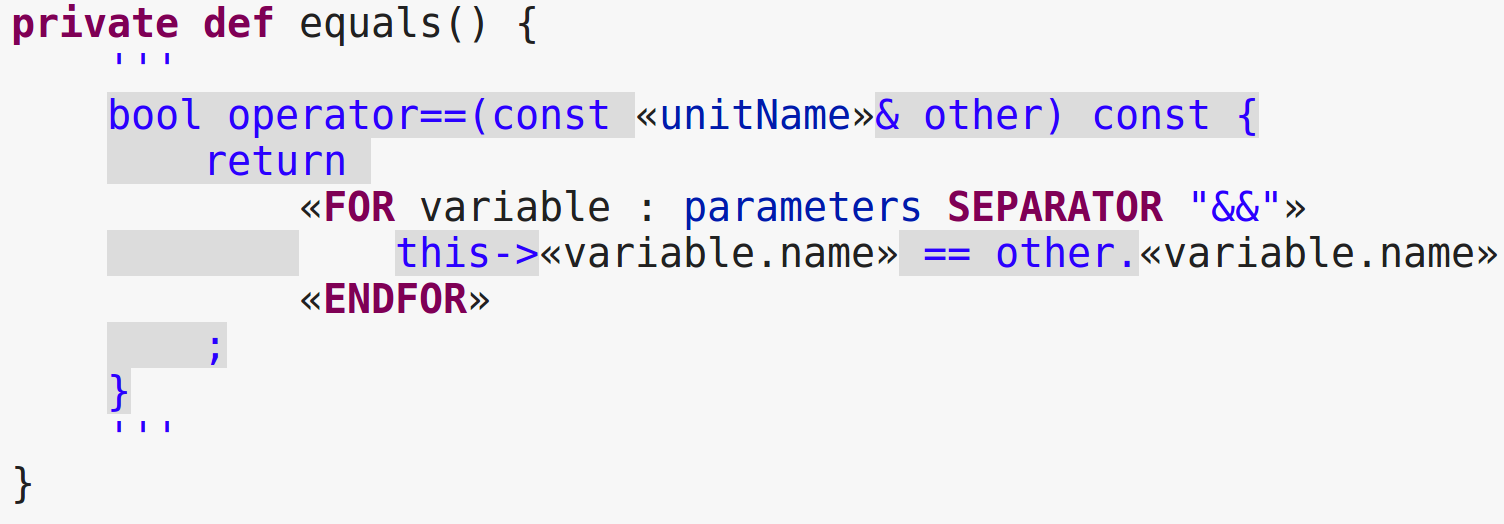
\includegraphics[width=0.8\textwidth]{figures/xtend.png}
		\caption{Template expressions with useful syntax highlight }
		\label{fig:xtend}
	\end{center}
\end{figure}


\subsection{\protect\cpptt }
The generated code is in \cpp{}, because it can be used in various platforms from embedded systems to high powered computers, or virtual machines in clouds. 
Efficiency also considered when choosing \cpp{}, so using embedded systems can be feasible. 

As modern \cpp{} is used in the framework, compiling the code requires a compiler supporting the \cpp{}14 standard.
We use various of modern \cpp{} elements, such as threads, mutexes, lambdas, smart pointers.
Non-generated code also uses templates to handle generated classes, this feature of C++ is extremely useful to integrate the generated code into the framework at compile time.

\section{ Build tools }

To build the generated sources and the \cpp{} libraries we developed, we use Make and CMake utilities. 


Make is a low-level build automaton tool. 
The build is configured by a file called the Makefile.
A Makefile consists of rules. 
A rule has targets (The artifacts generated by the rule), dependencies (artifacts, that must be created to run the rule), and a list of commands, that creates the target artifacts. 
From this declarative configuration file Make can decide the order which commands to run in which order to create a target artifact or multiple target artifacts.
If only some files changes Make only executes the required commands based on timestamps of the files.

As Make is only used in linux systems and larger Makefiles are hard to maintain, we use CMake.
CMake is a higher level tool for build automation. 
It is cross-platform, as CMake configuration files are processed and compiles into project files, like Visual Studio, or Xcode projects, or build scripts for Make or NMake.


\section{Protocol Buffers (Protobuf)}
Protocol Buffers (Protobuf) are a language-neutral, platform-neutral extensible mechanism for serializing structured data \cite{protobuf}. 
We use Protobuf to serialize the data and the messages in query execution.

Protobuf can be used by defining the message structure in \texttt{.proto} files and generating code from them to various languages, which code provide tools for creating, altering, serializing and deserializing messages.

In the framework, message definition for query execution is defined manually, while other messages, that are needed for specific query exeutions are generated by the framework.


\section{DDS -- Data Distibution Service}

DDS~\cite{DDS} is a data exchange standard for real-time systems. 
Its usage is publish-subscribe based.
DDS uses topics which is a relation of corresponding data elements. 
A key specifies the 

We use it to synchronize object and reference creation between computing units of the system.


\section{EMF -- Eclipse Modeling Framework}

Eclipse Modeling Framework is a modeling framework and code generation facility for building tools and other applications based on a structured data model.\cite{emf}.



They are based on Eclipse Modeling Framework (EMF), which provides modeling tools for eclipse based applications.

EMF defines an UML dialect called


\section{\protect\viatra{} }


\viatra{} \cite{viatra} is a framework for model transformations and model querying. 
It provides VQL (Viatra Query Language), a language for graph pattern definition.
\viatra{} can use local search-based and an incremental algorithms to provide matchings for graph patterns. 

In the framework we use the local search planner of \viatra{} and fine tune it to create plans more suitable for our purposes.











%----------------------------------------------------------------------------
\chapter{Preliminaries}
%----------------------------------------------------------------------------



\section{Modeling using graphs}

Structural and behavioral modeling of systems are often done using graphs. Graphs are useful abstraction as they are easy to understand, intuitive to use, and lots of existing algorithms can be used to process them.

\section{Runtime modeling}

In this framework, we use structural modeling to model the current state of the system. This model is called the live model, which captures the state and the operating context of the system. We monitor the system through this model: The model is updated with sensor data and information from other sources, so the model represents the physical system's latest state. 

\section{Graph pattern matching concepts}

A graph pattern's purpose is to define a list of variables, representing nodes, and a set of constraints for those variables. Some of the possible constraints are:

\begin{itemize}
	\item Type constraint -- a given node must be an instance of a type
	\item Reference -- a given reference must exist between two node
	\item Equality -- two variable must be the same
	\item Pattern match -- a subset of variables match to another graph pattern
	\item Negative application condition (NAC) -- a subset of variables must not match to another graph pattern
\end{itemize}
A list of vertices is called a \emph{match}, if binding them to the variables causes the constraints to be true.


\begin{figure}[h]
	\begin{center}
		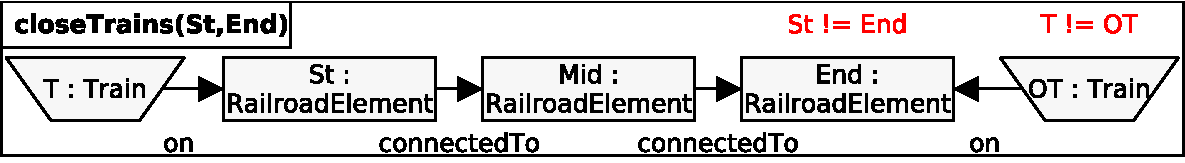
\includegraphics[width=0.75\textwidth]{figures/pattern-visual.pdf}
		\caption{Non-formal visual representation of a graph pattern}
		\label{pattern-visual}
	\end{center}
\end{figure}


\section{Local search}

Local search~\cite{bur-marton-msc} is an algorithm to provide matchings of a graph pattern in a graph. It is a depth-first search in the space of variable bindings. In the root of the search tree all the variables are unbound. Then with each constraint, we add a new level for the tree. The child of a variable binding is all the other variable binding where 
\begin{itemize}
	\item The bound variables of the parent are bound to the same values as the corresponding variable in the child
	\item The constraint is satisfied by the child
\end{itemize}

The search tree can be traversed without materializing it with depth-first search. This means, that the elements of the search tree are calculated on the fly, by modifying the parent variable binding.

To optimize the size of the search tree the order of the constraints must be chosen properly. 

\section{Distributed platform}

% adatok diszjunkt halmazokra bontva különböző csomópontra
% az algoritmusok is elosztottak, nem lesz összegyűjtve az infó, úgy van kiértékelve, hogy nincs aki mindent látna a rendszerből

As cyber-physical systems are distributed we must deal with the sensor data coming from different sensors at different computation units of the system. Sending the sensor data to one computation unit and evaluate on that cause different problems: Sensor data can be huge to send it through the network, the central node can be a SPOF, etc. In the presented framework the live model is distributed on the different computation units and the graph pattern matching algorithm itself runs in a distributed way. This eliminates the problem of central computers, but introduces complexity, that we must handle. 










%----------------------------------------------------------------------------
\chapter{Overview of the approach}
%----------------------------------------------------------------------------

%%
%% Futásidejű dolgok és kódgenerálás is!
%%


\begin{figure}[h]
	\begin{center}
		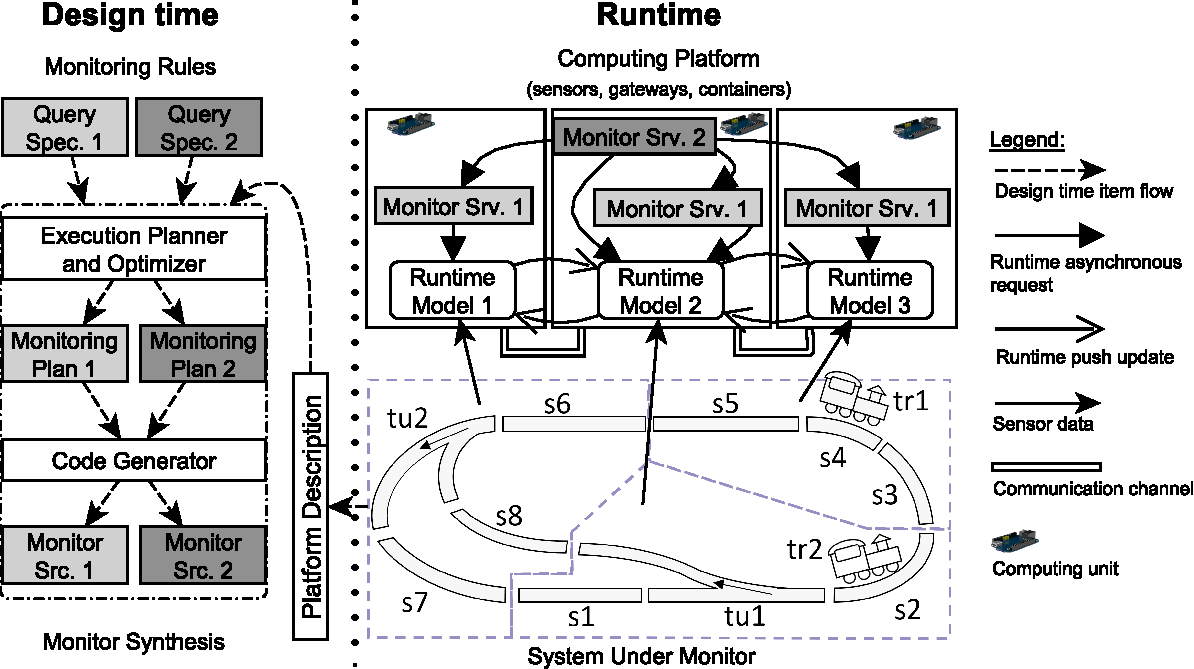
\includegraphics[width=\textwidth]{figures/fase-overview-crop.pdf}
	\end{center}
\end{figure}




%%
\chapter{Domain modeling and monitoring goal definition in EMF and \viatra{}}
%%

In this chapter the creation of initial artifacts is presented: domain models and graph patterns.
Domain modeling is an essential part of our framework, as the domain model defines the structure of the runtime live model, and affects the whole process. 
After the domain model is known, graph pattern can be specified, which will be used later in runtime analysis.
In the framework domain modeling are technologically backed up by EMF (Eclipse Modeling Framework), 
while graph pattern definition and processing are provided by \viatra{}.

\section{Eclipse Modeling Framework}


\begin{figure}
	\begin{center}
		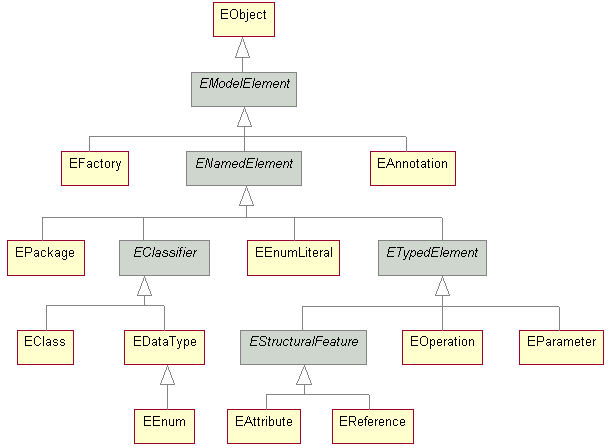
\includegraphics[width=0.5\textwidth]{figures/EcoreHierarchy.png}
		\caption{Hierarchy of Ecore elements (Source: \cite{ecore-package}) }
		\label{fig:ecore-hierarchy}
	\end{center}
\end{figure}

\begin{figure}
	\begin{center}
		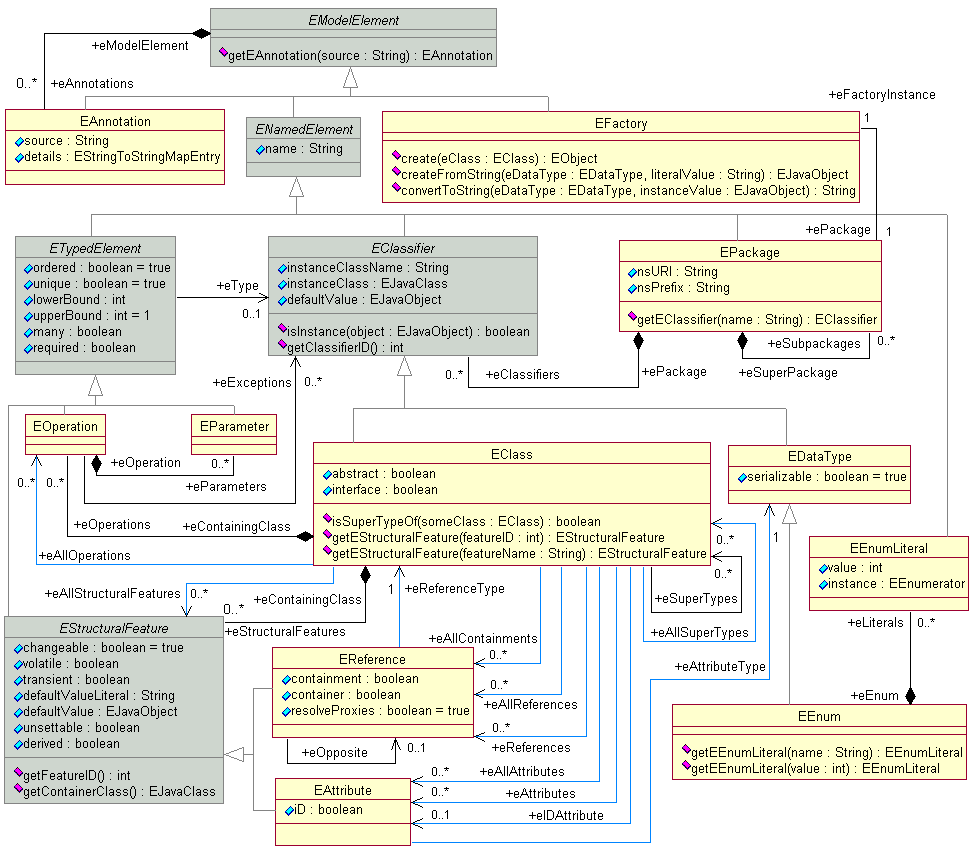
\includegraphics[width=\textwidth]{figures/EcoreRelations.png}
		\caption{Relations between Ecore elements (Source: \cite{ecore-package}) }
		\label{fig:ecore-relations}
	\end{center}
\end{figure}

Eclipse Modeling Framework (EMF) is an Eclipse based technology, which provides tools for model based developement: 
Ecore \cite{ecore-package} for metamodeling (Ecore actually defines a meta meta-model for metamodeling), and various tools like java code generation from ecore models, etc.

Ecore metamodeling is highly similar to defining class diagrams in UML, however, 
Ecore is more suitable for data and structural modeling: Interfaces are not a part of it, even though it can be substituted by abstract classes, as multiple inheritance is supported.

The hierarchy of Ecore elements can be seen on figure \ref{fig:ecore-hierarchy}, while its structure on \ref{fig:ecore-relations}
EObject is a base for everything, and its main purpuse to define the containment hierarchy of the model. 
EObjects can contain each other in a strict tree structure, circular containments are not permitted.
EModelElement expands EObject by giving the possibility to annotate them.

An Ecore model contains packages (EPackage). 
Packages have a namespace URI (nsURI), which can be used to refer it in other context eg.\ Viatra graph pattern definition.
Packages can contain other subpackages, classes (EClass), enumerations (EEnum), and data types (EDataType).

Classes have structural features: references and attributes (EStructuralFeature, EReference, EAttribute); also they have operations (EOperation).
References and attributes have multiplicity, defining their lower and upper bound is also possible.
ECore also provides tools to define containment hierarchy in the domain model itself: References can be containment or containing reference (considering direction of the reference). 
Two way navigation can be achieved by defining two reference and set them as the EOpposite of each other. A reference cannot be the EOpposite of itself, but its not a problem in most of the cases (eg.: \texttt{Human} class and \texttt{Spuse} reference). 

Multiple inheritance is supported for classes (eSuperTypes refers to direct base classes, and eAllSuperTypes for all transitively inherited base classes).

Besides classes, packages can contain enumerations and data types. 
Basic data types -- like EString, EInt, EBoolean etc.\ -- are defined by EMF, so its mostly never necessary to define others.
Enumerations are consists of EEnumLiterals. 
EEnumLiterals have an integral unique value, and its name is encapsulated in its EEnumerator instance.



	

\section{\viatra{} query language (VQL)}

As stated before, graph patterns can be defined using \viatra{} query language (VQL). 
The language syntax is simple, altough complex queries are not always self evident how to be expressed.

\subsection{Pattern definition}
Patterns and its bodies can be given by the \emph{pattern} keyword. 
Parameters must be specified after the parameter name in round brackets. 
Bodies of the pattern are given in curly brackets, separeted by the \emph{or} keyword

\begin{minipage}{\textwidth}
\begin{lstlisting}[language=vql]
pattern patternName( p1: Type1, p2: Type2){
... // Constraints for first body
} or {
... // Constraints for second body
} ...
\end{lstlisting}
\end{minipage}


\subsection{Constraints}
Constraints are given like statements. 
Each constraint is followed by a semicolon.

\vspace{\abovedisplayskip}
\begin{minipage}{\textwidth}
Type constraint can be given by specifying the type, then the object in round brackets.
\begin{lstlisting}[language=vql]
pattern patternName( o ){
	Type(o);
}
\end{lstlisting}
\end{minipage}
\vspace{\belowdisplayskip}

\begin{minipage}{\textwidth}
Reference constraint can be given by specifying which type's which reference must be checked, then giving the source and target variables in round brackets:
\begin{lstlisting}[language=vql]
pattern patternName( p1: Person, p2: Person ){
	Person.friend(p1, p2);
}
\end{lstlisting}
\end{minipage}
\vspace{\belowdisplayskip}

\begin{minipage}{\textwidth}
Other patterns can be used as constraint with the find keyword:
\begin{lstlisting}[language=vql]
pattern patternName( p1: Type1, p2: Type2, p3: Type3 ){
	find otherPatternName(p1, p2);
	find otherPatternName(p2, p3);
}
\end{lstlisting}

Also we can use underscore instead of specifying parameters. 
This way the constraint is satisfied, if the pattern matches with anything in the place of underscores (existential quantification).
\begin{lstlisting}[language=vql]
pattern patternName( p1: Type1 ){
find otherPatternName(p1, _);
}
\end{lstlisting}

This is the same as the following (if x is not used anywhere else):
\begin{lstlisting}[language=vql]
pattern patternName( p1: Type1 ){
find otherPatternName(p1, x);
}
\end{lstlisting}
\end{minipage}
\vspace{\belowdisplayskip}

\begin{minipage}{\textwidth}
Negative application condition can be expressed by neg find keyword:
\begin{lstlisting}[language=vql]
pattern patternName( p1: Type1, p2: Type2 ){
	neg find otherPattern(p1, p2);
	Type1.reference(p1, p2);
}
\end{lstlisting}

Also, we can use underscore if we don't want that the other pattern match occurs with \emph{any} value at the underscores. ( ie.\ neg find can be used to express negated existential quantification along with negated expressions )

\begin{lstlisting}[language=vql]
pattern patternName( p1: Type1 ){
	neg find otherPattern(p1, _);
}
\end{lstlisting}
\end{minipage}
\vspace{\belowdisplayskip}

\todo{Ez nem ugyanaz mint az előző esetben}

\begin{minipage}{\textwidth}
The keyword check can be used to create a constraint, that a given a java (XBase) expression is true. The expression only can refer to attribute  variables (Variables refering to data types instead of graph nodes).
\begin{lstlisting}[language=vql]
pattern adultPerson( p: Person ){
	Person.age(p, age);
	check(age >= 18);
}
\end{lstlisting}
\end{minipage}
\vspace{\belowdisplayskip}

\begin{minipage}{\textwidth}
The keyword eval can be used to evaluate a java (XBase) expression on attribute variables and assign the result to another variable.
\begin{lstlisting}[language=vql]
pattern patternName( p1: Person, p2: Person, agesum : EInt ){
	Person.age(P1, a1);
	Person.age(P2, a2);
	agesum = eval(a1 + a2);
}
\end{lstlisting}
\end{minipage}
\vspace{\belowdisplayskip}



\todo{ count find, equality, inequality}

\subsection{Annotations}


\section{VQL examples from the case study}

\todo{TODO megcsinalni}


\chapter{Graph pattern definition in \viatra{} query language (VQL)}

As stated before, graph patterns can be defined using \viatra{} Query Language (VQL). 
The language syntax is simple, altough complex queries are not always self evident how to be expressed.

\subsection{Pattern definition}
Patterns and its bodies can be given by the \emph{pattern} keyword. 
Parameters must be specified after the parameter name in round brackets. 
Bodies of the pattern are given in curly brackets, separeted by the \texttt{or} keyword

\begin{minipage}{\textwidth}
\begin{lstlisting}[language=vql]
pattern patternName( p1: Type1, p2: Type2){
... // Constraints for first body
} or {
... // Constraints for second body
} ...
\end{lstlisting}
\end{minipage}


\subsection{Constraints}
Constraints are given like statements. 
Each constraint is followed by a semicolon.

\vspace{\abovedisplayskip}
\begin{minipage}{\textwidth}
Type constraint can be given by specifying the type, then the object in round brackets.
\begin{lstlisting}[language=vql]
pattern patternName( o ){
	Type(o);
}
\end{lstlisting}
\end{minipage}
\vspace{\belowdisplayskip}

\begin{minipage}{\textwidth}
Reference constraint can be given by specifying which type's which reference must be checked, then giving the source and target variables in round brackets:
\begin{lstlisting}[language=vql]
pattern patternName( p1: Person, p2: Person ){
	Person.friend(p1, p2);
}
\end{lstlisting}
\end{minipage}
\vspace{\belowdisplayskip}

\begin{minipage}{\textwidth}
Other patterns can be used as constraint with the \texttt{find} keyword:
\begin{lstlisting}[language=vql]
pattern patternName( p1: Type1, p2: Type2, p3: Type3 ){
	find otherPatternName(p1, p2);
	find otherPatternName(p2, p3);
}
\end{lstlisting}

Also we can use underscore instead of specifying parameters. 
This way the constraint is satisfied, if the pattern matches with anything in the place of underscores (existential quantification).
\begin{lstlisting}[language=vql]
pattern patternName( p1: Type1 ){
find otherPatternName(p1, _);
}
\end{lstlisting}

This is the same as the following (if x is not used anywhere else):
\begin{lstlisting}[language=vql]
pattern patternName( p1: Type1 ){
find otherPatternName(p1, x);
}
\end{lstlisting}
\end{minipage}
\vspace{\belowdisplayskip}

\begin{minipage}{\textwidth}
negative pattern match can be expressed by \texttt{neg find} keyword:
\begin{lstlisting}[language=vql]
pattern patternName( p1: Type1, p2: Type2 ){
	neg find otherPattern(p1, p2);
	Type1.reference(p1, p2);
}
\end{lstlisting}

Also, we can use underscore if we don't want that the other pattern match occurs with \emph{any} value at the underscores. ( ie.\ \texttt{neg find} can be used to express negated existential quantification along with negated expressions )

\begin{lstlisting}[language=vql]
pattern patternName( p1: Type1 ){
	neg find otherPattern(p1, _);
}
\end{lstlisting}

It is very important to clarify, that unlike in the case of find this is \emph{not} the same as the following:

\begin{lstlisting}[language=vql]
pattern patternName( p1: Type1 ){
	neg find otherPattern(p1, x);
}
\end{lstlisting}
As this will match if there exist \emph{any} x, that (p1, x) not satisfies the \texttt{otherPattern}.


\end{minipage}
\vspace{\belowdisplayskip}



\begin{minipage}{\textwidth}
\texttt{count find} can be used to count maches to a given pattern (Counting the ways underscores can be bound to form a match for the other pattern)
\begin{lstlisting}[language=vql]
pattern personPattern(p){
	Person(p)
}

pattern countPersons(cnt)
	cnt == count find personPattern(_);
}
\end{lstlisting}
	
\end{minipage}
\vspace{\belowdisplayskip}



\begin{minipage}{\textwidth}
Equality and inequality also can be given between variables ( ==, != ):
\begin{lstlisting}[language=vql]
pattern friendsOfFriends(a, b){
	Person.friend(a, x);
	Person.friend(x, b);
	a != b;
}

pattern sameOrFriend(a : Person, b: Person){
	Person.friend(a, b);
} or {
	a == b;
}
\end{lstlisting}
	
Equality constraint is mostly used between parameters, as in other cases simply using one variable instead of using two and making them equal is simpler.  
	
\end{minipage}
\vspace{\belowdisplayskip}



\begin{minipage}{\textwidth}
The keyword \texttt{check} can be used to create a constraint, that a given java (XBase) expression is true. The expression only can refer to attribute  variables (Variables refering to data types instead of graph nodes).
\begin{lstlisting}[language=vql]
pattern adultPerson( p: Person ){
	Person.age(p, age);
	check(age >= 18);
}
\end{lstlisting}
\end{minipage}
\vspace{\belowdisplayskip}

\begin{minipage}{\textwidth}
The keyword \texttt{eval} can be used to evaluate a java (XBase) expression on attribute variables and assign the result to another variable.
\begin{lstlisting}[language=vql]
pattern patternName( p1: Person, p2: Person, agesum : EInt ){
	Person.age(P1, a1);
	Person.age(P2, a2);
	agesum == eval(a1 + a2);
}
\end{lstlisting}
\end{minipage}
\vspace{\belowdisplayskip}

\subsection{Annotations}

\begin{minipage}{\textwidth}
Annotations can be added to patterns with the following syntax:
\begin{lstlisting}[language=vql]
@AnnotationName(
	a = {p1, p3}
	a = {p2, p3}
	b = "A simple string"
)
@AnnotationName2
pattern patternName( p1, p2, p3, ... )
	...
\end{lstlisting}
\end{minipage}
\vspace{\belowdisplayskip}

An annotation has a name (after @), and some named attributes using \texttt{name = value} syntax inside parentheses.
One attribute name can used multiple times. 
The attribute's value can be a single value or a list of values, that can be strings, numerals, or parameter reference.


\subsubsection{Annotations used by our framework}

The framework can process two types of annotations:
\begin{itemize}
	\item \texttt{@Bind} can be used to control what kind of graph pattern matching code will be generated, ie.\ what parameter sets can be bind to restrict the results. The version of the query, where all the parameters are unbound are generated by default.
	
	\item \texttt{@SkipDefaultGen} can be used to avoid default query generation for unbound version, eg.\ in case of helper patterns, we would not want to use it by itself most of the time.
	
\end{itemize}


\section{VQL examples from the case study}
\label{sec:vql-examples}

To show how the these elements can be used in patterns, now we present the benchmarked queries, and what their semantics are, for this we show, what subgraphes these patterns matches from the graph depicted on \autoref{fig:query-example-model}. This simple model represents 3 sequence of railroad elements and a Turnout (7) between them.
\vspace{0.1\textwidth}


\begin{figure}[H]
	\begin{center}
		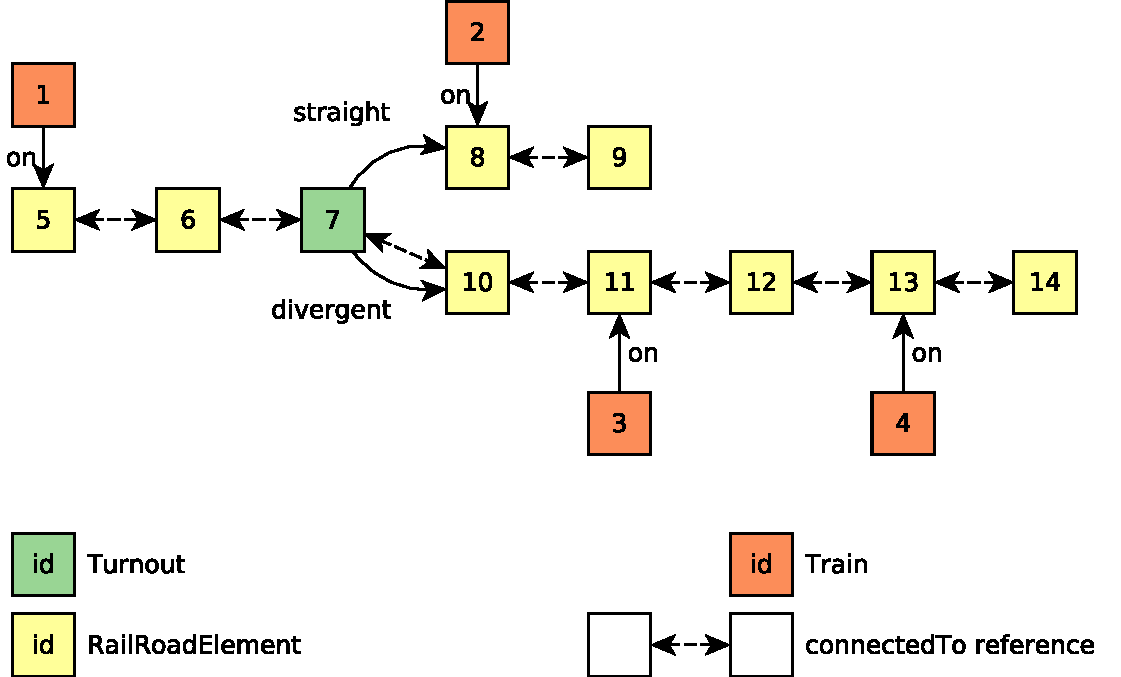
\includegraphics[width=\textwidth]{figures/query-example-model.pdf}
		\caption{Example model}
		\label{fig:query-example-model}
	\end{center}
\end{figure}

\subsection{\texttt{trainLocations}}
\begin{minipage}{\textwidth}

\texttt{trainLocations} pattern matches for all the (\texttt{train},\texttt{loc}) tuples where \texttt{train} is a Train, that is on the location \texttt{loc}.
Using this pattern we can query all the trains, and where they are.
As @Bind annotation denotes, we can also bind the train parameter: this way we can query where a specific train is.
\begin{lstlisting}[language = vql]
@Bind( parameters=train )
pattern trainLocations(train: Train, loc: RailRoadElement)
{
	Train.on(train, loc);
}
\end{lstlisting}

\begin{figure}[H]
	\begin{center}
		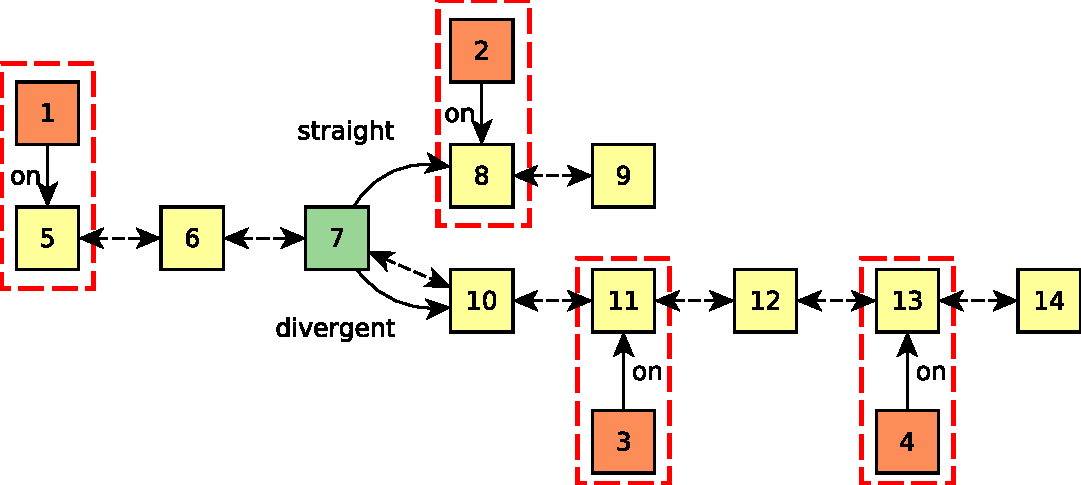
\includegraphics[width=0.8\textwidth]{figures/query-example-model-trainloc.pdf}
	\end{center}
\end{figure}

\end{minipage}






\subsection{\texttt{endOfSiding}}

End of siding pattern matches, when there is a last segment of railroad, and a trail is near to that segment.
The last segment is expressed as a segment, which has a neighbor, but only one.
If a train is on the neighbor, the pattern matches.

\begin{minipage}{\textwidth}
\begin{lstlisting}[language = vql]
pattern endOfSiding(train: Train, end: RailRoadElement, neighbor: RailRoadElement)
{
	RailRoadElement.train(neighbor, train);		
	RailRoadElement.connectedTo(end,neighbor);
	1 == count find connected(end,_);	
}
\end{lstlisting}

\begin{figure}[H]
	\begin{center}
		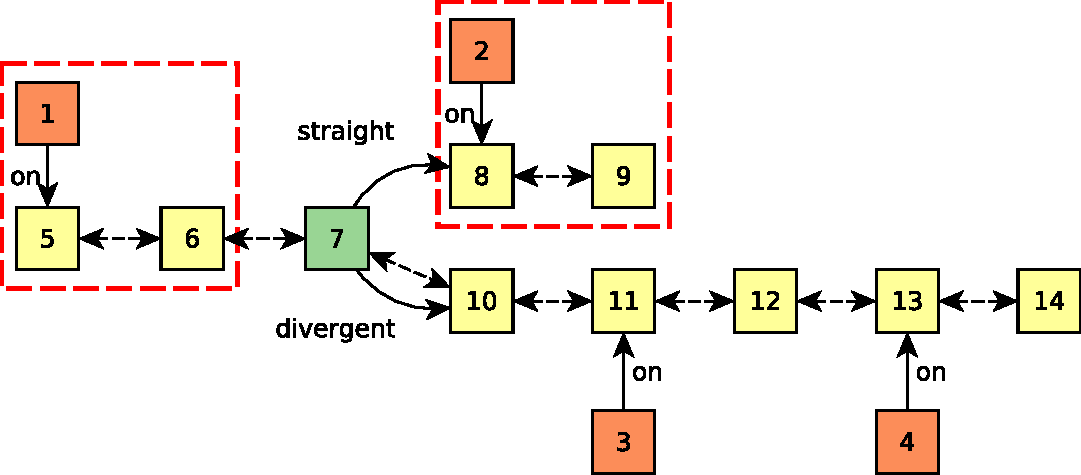
\includegraphics[width=0.8\textwidth]{figures/query-example-model-endofsiding.pdf}
	\end{center}
\end{figure}

\end{minipage}
\vspace{\belowdisplayskip}




\subsection{\texttt{derailment}}
\begin{minipage}{\textwidth}
	
\texttt{derailment} matches, when a train is on the non-connecting side of a turnout:
The turnout switches between the straight and the divergent railroad. 
connectedTo reference points to two segment: The selected segment and the third, always connecting segment.
So if a train is on a straight or the divergent segment (1, 2), but that segment does not connected to the turnout(3), then the pattern matches to this train and the segment it is on.


\begin{lstlisting}[language = vql]
pattern derailment(elem: RailRoadElement, train: Train)
{
	Turnout(turnout);
	RailRoadElement.train(elem,train); (1)
	find straightOrDivergent(turnout, elem) (2);
	neg find connected(elem, turnout); (3)
}

// Helper pattern, does not need to be generated, if not used
@SkipDefaultGen
private pattern straightOrDivergent(turnout : Turnout, elem : RailRoadElement){
	Turnout.straight(turnout, elem);
} or {
	Turnout.divergent(turnout, elem);
}

// We need this query, because negation can be only be expressed with neg find
@SkipDefaultGen
private pattern connected(a : RailRoadElement, b : RailRoadElement){
	RailRoadElement.connectedTo(a,b);
}

\end{lstlisting}

\begin{figure}[H]
	\begin{center}
		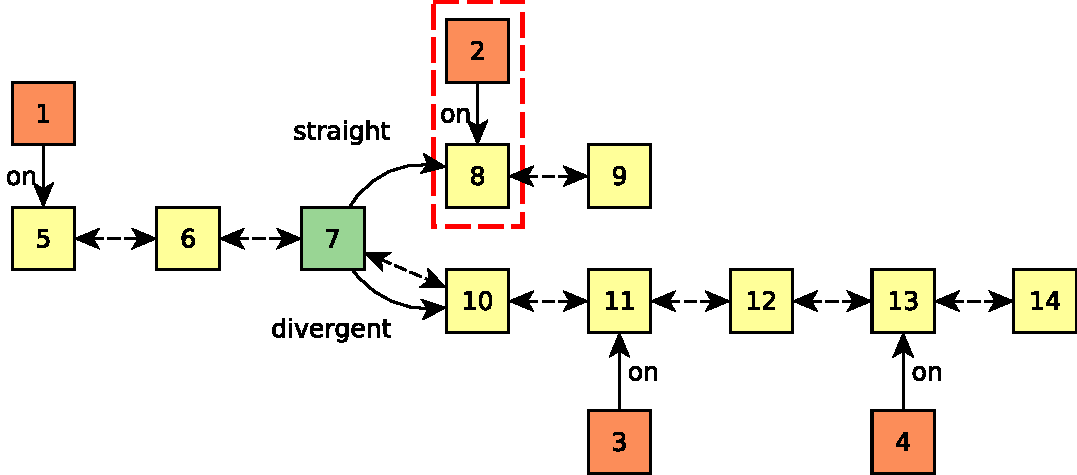
\includegraphics[width=\textwidth]{figures/query-example-model-derailment.pdf}
	\end{center}
\end{figure}


\end{minipage}
\vspace{\belowdisplayskip}







\subsection{\texttt{closeTrains}}
\begin{minipage}{\textwidth}
Two trains are close, if they are on two segments that are connected by another segment
\begin{lstlisting}[language = vql]
pattern closeTrains(start : RailRoadElement, end : RailRoadElement)
{
	Train.on(t1,start);
	
	RailRoadElement.connectedTo(start,middle); // Has EOpposite, inverse navigation is effective even without model index
	RailRoadElement.connectedTo(middle, end);
	
	Train.on(t2, end);
	
	start != end; // This ensures that the start and end segment is different
	
	t1 != t2; // A train may occupy two neighboring segments when moving; this is not a hazardous situation
}
\end{lstlisting}


\begin{figure}[H]
	\begin{center}
		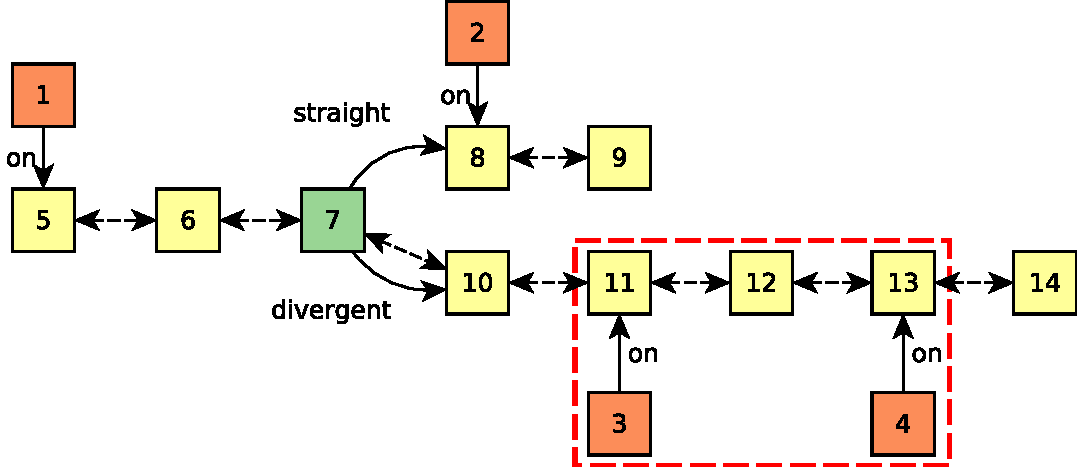
\includegraphics[width=\textwidth]{figures/query-example-model-closetrains.pdf}
	\end{center}
\end{figure}


\end{minipage}
\vspace{\belowdisplayskip}









%%
\chapter{Generating query based monitoring components}
%%

After the domain model of the system is designed, and the graph queries are written, the monitoring components can be generated and deployed along with \cpp{} tools for modeling the domain.
As stated before, domain modeling and graph query definition are done using EMF and \viatra{} technologies.
In this chapter, I present how the monitoring components are generated from these artifacts.

From the metamodel, the framework generates the classes, which enables the programmer to model the system's state in \cpp{}.
Also, we generate the monitoring code for the system, which is basically the \cpp{} version of the planned graph queries. 
These graph queries are evaluated on the maintained \cpp{} model.

\section{Generating classes from the metamodel}

The domain model consists of packages (EPackage), enumerations (EEnum) and classes (EClass).
From an EPackage, we generate a folder and every source file originated from the elements of the package will be generated in that folder. 
We generate sources from each class and enumeration of the package, also we generate other artifacts for the package.


\subsection{Mapping an EClass to \protect\cpp }


\todo{ábra szépítés}
\begin{figure}
	\begin{center}
		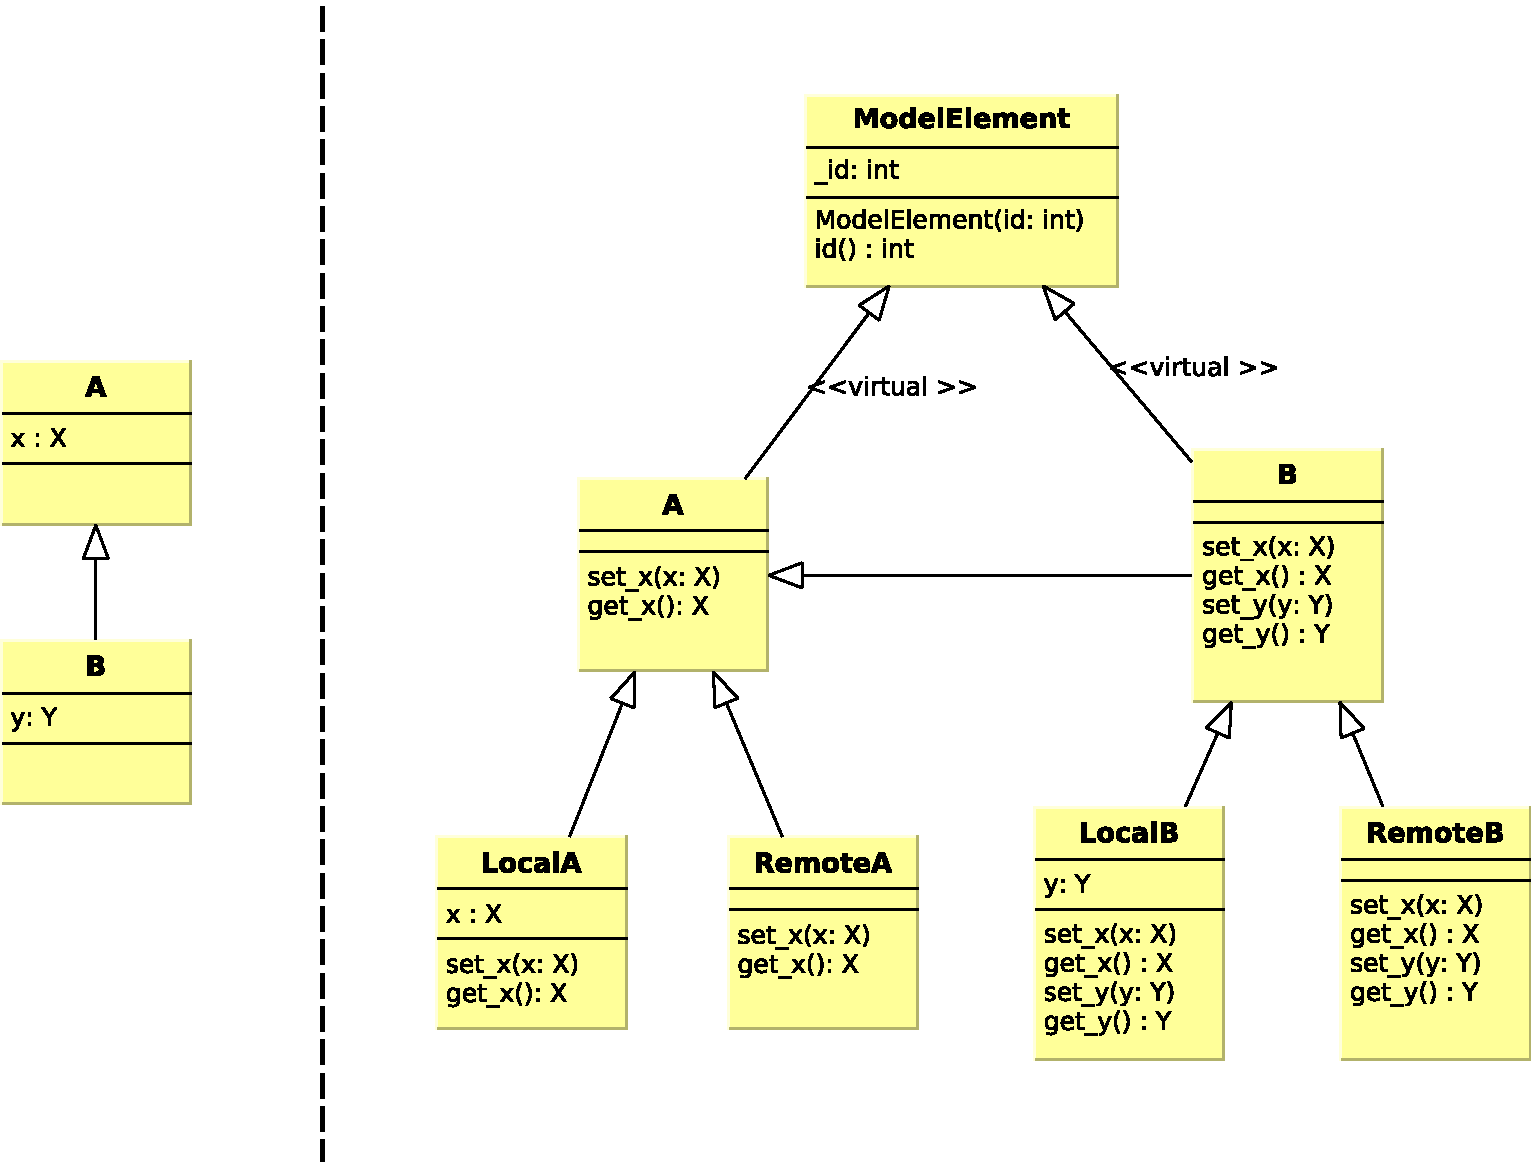
\includegraphics[width=\textwidth]{figures/eclass-to-cpp.pdf}
		\caption{Mapping of two EClasses, one inherited from the other (Left: EClasses, right: \protect\cpp{} classes) }
		\label{fig:eclass-to-cpp}
	\end{center}
\end{figure}


The EClasses of the metamodel are mapped to various \cpp{} classes, as depicted on \mbox{Figure~\ref{fig:eclass-to-cpp}}.
From each EClass we generate three \cpp{} classes:

\begin{itemize}
	\item An interface (abstract class with only pure virtual methods in \cpp{})
	\item A local class
	\item A remote class
\end{itemize}


The interface provides access to an instance of the EClass.
The local class implements the interface. It stores the attributes and references of the instances allocated to the local computing unit, and made them accessible by the methods of the implemented interface.
The remote class implements the interface, but are only used to substitute remote objects in references to them; 
Accessing its variables are not possible, because they are stored in another node. 

\subsection{Mapping an EEnum to \protect\cpp }

Enumerations are simply mapped to \cpp{} enum classes as depicted on Fig.\ref{fig:eenum-to-cpp}.

\begin{figure}[H]
	\begin{center}
		
		\begin{minipage}[c]{\textwidth}
		\begin{minipage}[r]{0.52\textwidth}
			\hfill
			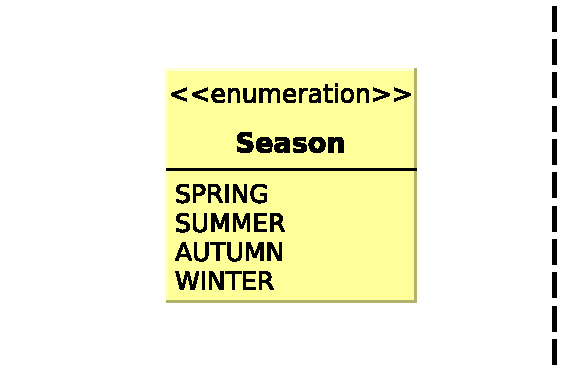
\includegraphics[width=0.735\textwidth]{figures/eenum-to-cpp.pdf}
		\end{minipage}
			\hspace{0.05\textwidth}
		\begin{minipage}[c]{0.25\textwidth}
\begin{lstlisting}[language=C++]
namespace Package{

enum class Season{
	SPRING = 0,
	SUMMER = 1,
	AUTUMN = 2,
	WINTER = 3
};

}
\end{lstlisting}			
		\end{minipage}
		\end{minipage}
		\caption{Mapping of an enumeration to \protect\cpp{} enum class }
		\label{fig:eenum-to-cpp}
	\end{center}
\end{figure}

\subsection{ Generating ModelRoot class and utilities }


\todo{MEGÍRNI}





\section{Overview of the query compilation workflow}

The compilation of the queries of the CPS is depicted in fig. \ref{figure:query-compile-workflow}. 
First, vql files are parsed using EMF so its content is loaded into a Pattern Model.
The Pattern Model are processed by \viatra{} and converted into PSystem representation of queries.
After that, we extend this representation with type information, as type information is important in the \cpp{} generated code.
Then, we create the plan for query execution; We use the local search planner of \viatra{} fine tuned with our search operation cost function to improve performance of distributed queries. 
We also use some optimizations later to improve distributed performance. 
After the fully optimized plan is ready, we can construct the generator model describing the source code structure and generate the \cpp{} files.


\begin{figure}[h]
	\begin{center}
		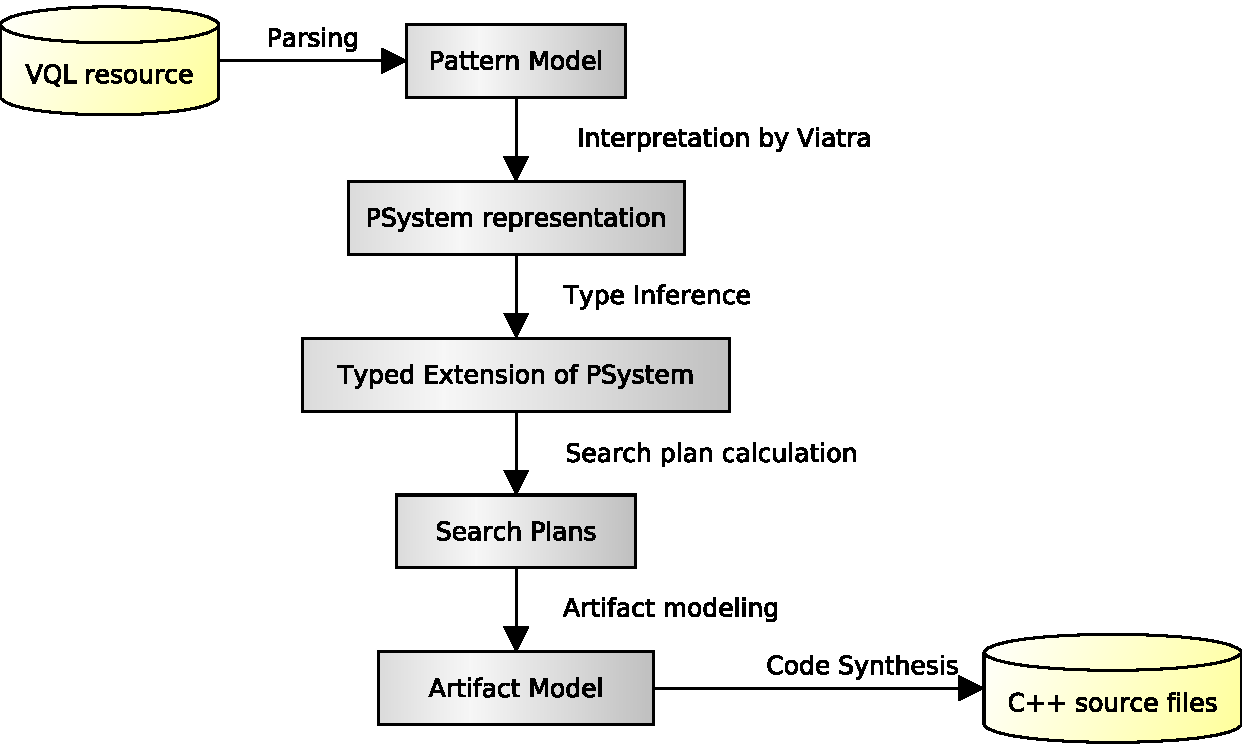
\includegraphics[width=0.8\textwidth]{figures/query-compilation-workflow.pdf}
		\caption{Query compilation workflow}
		\label{figure:query-compile-workflow}
	\end{center}
\end{figure}



\section{Viatra plan}

The query file is processed by \viatra{}~\cite{viatra} and a local search plan is generated. 
The local search planner of \viatra{} can be customized by specifying a cost function
In case of local search, the plan is a sequence of search operation defined as an application of a constraint.

\section{Completed plan}

\viatra{} generated plans are not intended for external usage. 
We need to complete it with additional information to use it for our purposes. 
One of the main concern is type information. To obtain type information we use the constraints to deduce the type of a variable. 


\section{Additional optimization}

After we complete the plan with type information and other details, it can be used to generate C++ code, although before that step we use further optimizations. 
These optimizations considers distributed execution of the plan, so it can improve the plan generated by \viatra{} which is generated to be used in a single computer.


\subsection{Replace pattern calls with simpler operations}
There are some cases, where helper patterns are simple, and used to define simple conditions. 
In this case, evaluationg the subquery is not always the most efficient method, sometimes these can be replaced by simple search operations:

\subsubsection{Reference Pattern}
We use the phrase \emph{reference pattern} for a pattern with 2 parameters if its only constraint is that a reference exist between the two parameters, eg.:
\begin{lstlisting}[language = vql]
private pattern connected(a : RailRoadElement, b : RailRoadElement){
	RailRoadElement.connectedTo(a,b);
}
\end{lstlisting}

In the following examples i will use this query as an example to demonstrate how the application of this query can be replaced by an other operation.

\subsubsection{Counting reference pattern}
\begin{lstlisting}[language = vql]
1 == count find connected(a, _);
\end{lstlisting}


\subsubsection{Negative application of a reference pattern}

\begin{lstlisting}[language = vql]
neg find connected(a, _);
\end{lstlisting}

\subsection{Filter unnecessary operations, checks}
As the original plan is generated by the localsearch planner of \viatra{}, there can be redundant operations, which can be ommited. This includes:

\begin{itemize}
	\item Check operation -- The generated code is strongly typed, so we don't need type checks in most cases, unlike in the Java implementation, where the tuples contains plain java objects with unknown types.
	
	\item Distribution operations -- \todo{KIFEJTENI}
\end{itemize}



\section{C++ code generation}

The completed and optimized plan are used to generate \cpp{} code. 
Two main methods can be used to run local search plan in case of generated code. 
One is to generate the plan as a data structure and create an interpreter that uses that plan to find matches. 
The other is to generate the code directly from the plan. 
The first method is good if we want to change the plan at runtime, but the interpreter itself introduces an overhead, causing performance to be slower.
We used the later, because we don't change the plan at runtime.















%%%%
%%%%
%%%%
\chapter{Query compilation workflow}
%%%%
%%%%
%%%%

After the model handling code is generated, the user of the framework can build and maintain the live model at runtime. 
Still to use find matches for graph patterns, we need additional components to be generated. 
In this chapter, we show the workflow of query code generation in the framework. 


\begin{figure}[H]
	\begin{center}
		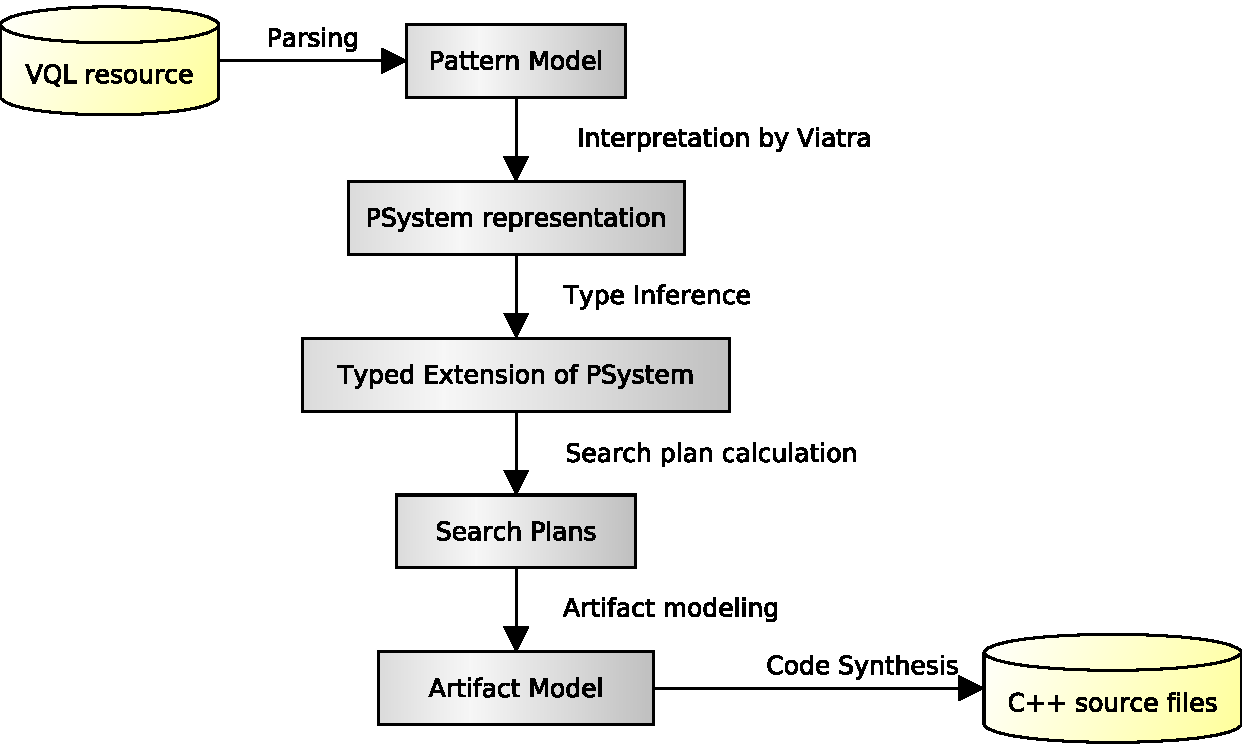
\includegraphics[width=\textwidth]{figures/query-compilation-workflow.pdf}
		\caption{Query compilation workflow}
		\label{figure:query-compile-workflow}
	\end{center}
\end{figure}


\section{Overview}

The compilation of graph patterns is depicted in fig. \ref{figure:query-compile-workflow}:

\begin{enumerate}[(1)]

\item 
First, VQL files containing the patterns are parsed using EMF so their contents are loaded into a Pattern Model.
\item 
The Pattern Model is processed by \viatra{} and converted into PSystem representation of queries.
\item 
After that, we extend this representation with type information, as type information is more important in the \cpp{} generated code, than in the \viatra{} implementation.
\item 
Then, we create the plan for query execution; we use the local search planner of \viatra{} fine tuned with our search operation cost function to improve performance of distributed queries. 
We also use some optimizations later to improve distributed performance. 
\item 
After the fully optimized plan is ready, we can construct the generator model describing the source code structure 
\item
and generate the \cpp{} files from them.

\end{enumerate}



\section{PSystem representation}


The VQL file is loaded into a PatternModel. 
The framework does not use this representation, but passes it to \viatra, which creates its own representations of it called PSystem. \cite{psystem}. 


\begin{figure}[H]
	\begin{center}
		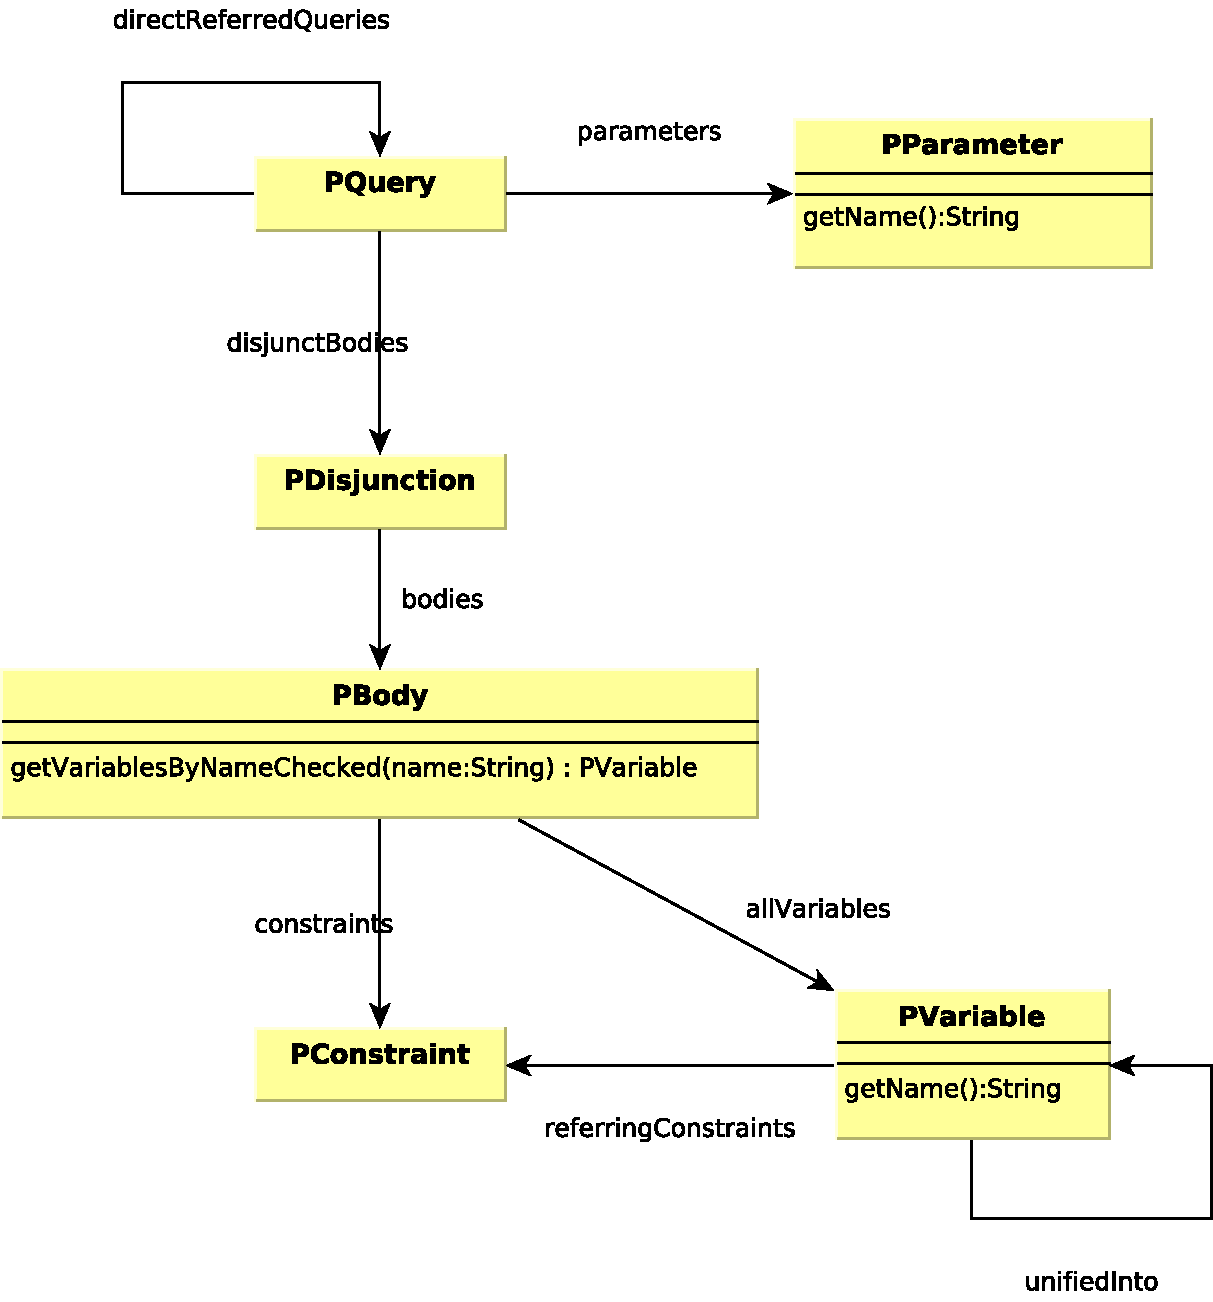
\includegraphics[width=0.6\textwidth]{figures/psystem.pdf}
		\caption{PSystem's basic structure}
		\label{fig:psystem}
	\end{center}
\end{figure}

The structure of PSystem representation is shown on \autoref{fig:psystem}. 
As their implementation is hidden behind interfaces, most of the refrences means getter functions (In Xtend, getter functions can be used with field access syntax like \csharp{} properties). 
Graph patterns are represented by a PQuery. 
A PQuery has a parameter list. 
The most important attribute of parameters are its names. 
A PQuery consists of a PDisjunction, which consists of a set of PBodies. 
PDisjunctions play role in Query rewriting, where the bodies of a PQuery gets optimized, or changed other ways.
PBody consists of PConstraints. 
PConstraint is a basic interface for various constraints. 
Altough constraints refer to variables, all variables in a PBody can be accessed from PBody.

%A variable can be unified into another variable. 
%This can happen when equality constraint is used between two variable: 
%Equality constraint is omitted, one of the variable gets unified into the other, and other constraints do not have to be changed.



\section{Typed Extension of PSystem}

We extend PSystem with additional information, mainly with type information for variables and parameters.
For this the types of the variables and parameters must be infered based on type constraints of the graph pattern.

First the types of the variables must be infered. 
\begin{enumerate}
	\item 
	First, we collect all the type constraints, that the variable must satisfy.
	We do this, by collecting all the variables that are the same as the variable( via equality constraints ), 
	then collect the constraints refering to them.
	From this we can create the set of candidate types.
	\item
	Then we choose the type:
	\begin{itemize}
		\item
		If all the types are compatible data types (integral types, or the same type), then we choose the most specific type
		\item
		If all the types are EClass types, then we select the most general class, that is compatible (extends it or is the same) of all the classes and choose that.
		If we cannot choose such EClass, or there are multiple classes that satisfies this, then the type inference is failed.
		A case for this is depicted on \autoref{fig:multiple-inheritance-problem}: if a variable's type is restricted as \texttt{A} and \texttt{B}, we cannot choose between \texttt{X} and \texttt{Y}
		\item
		In other cases (e.g. both of data types and class types is used) the type inference is failed
	\end{itemize}
\end{enumerate}


\begin{figure}[h]
	\begin{center}
		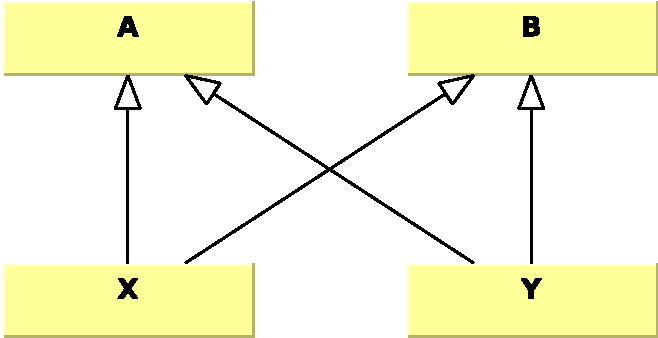
\includegraphics[width=0.4\textwidth]{figures/multiple-inheritance-problem.pdf}
		\caption{One of the problems with type inference in case of multiple inheritance}
		\label{fig:multiple-inheritance-problem}
	\end{center}
\end{figure}

If the types of the variables are known then the types of the parameters can be inferred. 
For this, we collect the variables that represent this parameter from each body.
As the parameters value can be any of the variable, we choose the type, that generalizes them.
If no such type exists, the inference of the parameter type is failed.

We also maintain additional information in our representation. 
Bodies also maintain the relationship between variables and parameters. 
In PSystem, this information is not directly available, parameters and variables need to be matched by name.

\section{Search plan calculation}

\subsection{Creating a basic plan}
After we have extended PSystem with the needed information, we can plan how the pattern will be evaluated at runtime, i.e.\ how the query code will process the graph and produce matches for the pattern.

The first step is flattening and normalization. 
The purpose of flattening is to replace pattern calls with the constraints of the bodies of the referenced pattern, as in most of the cases this leads more efficient code, than handling the pattern as a black box.
At normalization, equality constraints are optimized: equal variables are unified, and equality constraint is omitted.

After flattening and normalization, we need to create the search plan for each body of the pattern. From a set of constraints that declaratively defines the body we need to create an imperative sequence of search operations.

For this, we use the local search planner of \viatra{}.
This planner takes a pattern and a cost function, then creates a permutation of constraints that minimizes the cost function. 
The cost function gives an approximated cost of applying a constraint based on the variables bound before the application and other information\footnote{One of the used detail is the statistics on the instance model: As it can only be available at runtime, we can't use these at design time}. 
After this permutation is achieved, then search operations will be created by mapping the constraints to them considering their position.

For the different types of constraint applications we use the following search operations. We also give the basic search operation a name to use them later in the examples.


\subsubsection{Equality and pattern find}
These two types of constraints are never appear in this phase, as they are both optimized. Pattern find constraints are replaced with their inner constraints in the flattening phase, while Equality constraints are optimized in normalization phase.


\subsubsection{Type constraint}
We apply a type constraint the following way:

\begin{itemize}
\item If the variable is bound, we need to check whether the already bound value is of that type, we denote this CheckInstanceOf(Var, Type).
\item If the variable is unbound, we need to iterate over the instances of the type and follow the algorithm, we denote this ExtendInstanceOf(Var, Type) ).
\end{itemize}


\subsubsection{Reference and attribute (Structural feature) constraint}

Reference and attribute relations are called structural features.
We apply the constraint of a structural feature the following way:
\begin{itemize}
	\item If the source and target variable is bound too, then we just checks, whether the constraint is satisfied by those constraint. 
	
	\mbox{(CheckNavigation(from, to, structural feature))}
	\item If the source variable is bound and the target is unbound, then we extend along using the source variable for all its elements (or single element, if it does not have multiplicity). 
	
	\mbox{(ExtendNavigation(from, to, structural feature))}
	\item If the target variable is bound and the source is unbound, then we check, if the structural feature is a reference having an opposite reference. 
	\begin{itemize}
		\item If it is, then we can navigate along the opposite reference, so we can use it to extend to the source variable. 
		
		\mbox{ExtendNavigation(to, from, opposite structural feature)}
		\item If not, we add two search operation: 
		
		ExtendInstanceof(type of src, src), CheckNavigation(src, target). 
	\end{itemize}

	\item If both of  target variable and the source is unbound, then we use the next 2 search operation: ExtendInstanceof(type of src, src), ExtendNavigation(src, target)

\end{itemize}


\subsubsection{Negative pattern call and transitive closure}

We only apply these constraints, when all the referred variables are bound, so we only compile them into check operations:
\begin{itemize}
	\item Negative pattern application $\rightarrow{}$ NegativePatternCheck(pattern, $v_1$, $v_2$, \dots{} )
	\item Transitive closure $\rightarrow{}$ BinaryTransitiveClosureCheck(pattern, $v_1$, $v_2$).
\end{itemize}

\subsubsection{Count pattern matches}

This constraint can be applied, when all the variables given to the sub pattern as parameter are bound. 
The count of the matches is stored in another variable. 
We choose the search operation based on this variable.

\begin{itemize}
	\item If this variable is bound, then we create a check operation: 
	CheckPatternMatchCounter(countVar, pattern, $v_1$, $v_2$, \dots{})
	\item If this variable is not bound, then we create an extend operation: 
	ExtendPatternMatchCounter(countVar, pattern, $v_1$, $v_2$, \dots{})
\end{itemize}


\subsubsection{Inequality}
Inequality is only supported as a check operation: CheckInequality(x, y)


\subsection{Expanding the plan for distributed evaluation}
Now the sequence of search operation can be used to find the matches of a pattern on a single computer, but in a distributed setup, we need additional steps to make the plan correct.
The following search operations can cause problems in a distributed setup:
\begin{itemize}
	\item CheckNavigation	
	\item ExtendNavigation
	\item ExtendInstanceOf
\end{itemize}

CheckNavigation and ExtendNavigation need the source object to be available at the computing unit, because references and attributes are stored on local objects.
ExtendInstanceOf needs to expa

\subsubsection{Example for search plan creation on a pattern }
\todo{examplet csinálni ide}


\subsection{Additional optimization}

After we complete the plan with type information and other details, it can be used to generate C++ code, although before that step we use further optimizations. 
These optimizations considers distributed execution of the plan, so it can improve the plan generated by \viatra{} which is generated to be used in a single computer.


\subsubsection{Replace pattern calls with simpler operations}
There are some cases, where helper patterns are simple, and used to define simple conditions. 
In this case, evaluationg the subquery is not always the most efficient method, sometimes these can be replaced by simple search operations:

\paragraph{Reference Pattern}
We use the phrase \emph{reference pattern} for a pattern with 2 parameters if its only constraint is that a reference exist between the two parameters, eg.:
\begin{lstlisting}[language = vql]
private pattern connected(a : RailRoadElement, b : RailRoadElement){
	RailRoadElement.connectedTo(a,b);
}
\end{lstlisting}

In the following examples i will use this query as an example to demonstrate how the application of this query can be replaced by an other operation.

\paragraph{Counting reference pattern} 
Instead of counting a reference pattern bounding the source variable, we can insert a search operation counting the references.

\begin{lstlisting}[language = vql]
1 == count find connected(a, _);
\end{lstlisting}


\paragraph{Negative application of a reference pattern}
Instead of checking wether a reference pattern matches we can simply create a search operation which checks the existence of the reference.
\begin{lstlisting}[language = vql]
neg find connected(a, _);
\end{lstlisting}

\todo{Lesz itt egy összefoglaló táblázat ezekről mindről}


\subsubsection{Filter unnecessary operations, checks}
As the original plan is generated by the localsearch planner of \viatra{}, there can be redundant operations, which can be ommited. This includes:

\begin{itemize}
	\item Check operation -- The generated code is strongly typed, so we don't need type checks in most cases, unlike in the Java implementation, where the tuples contains plain java objects with unknown types.
	
	\item Distribution operations -- We also need to detect redundant distribution operations, this can happen, when we know, that a certain object is local after the previous operation.
\end{itemize}



\section{\protect\cpptt{} code generation}



\subsection{Generated code structure}

The structure of the generated code is depicted on \autoref{fig:generated-code-structure-perpattern}.
For each pattern we generate a \texttt{Matcher} class.
This class contains the methods for query execution.
We also generate a \texttt{Match} class which is a data class for pattern match.
A \texttt{MatchSet} class is also generated which holds a subresult of a query, which is a collection of matches.
We generate \texttt{Frame} classes, which can holds variable bindings. 
Since different parameter-bound patterns and different bodies of a pattern can contain a different set of variables, we generate multiple frame class for a pattern.


\begin{figure}[h]
	\begin{center}
		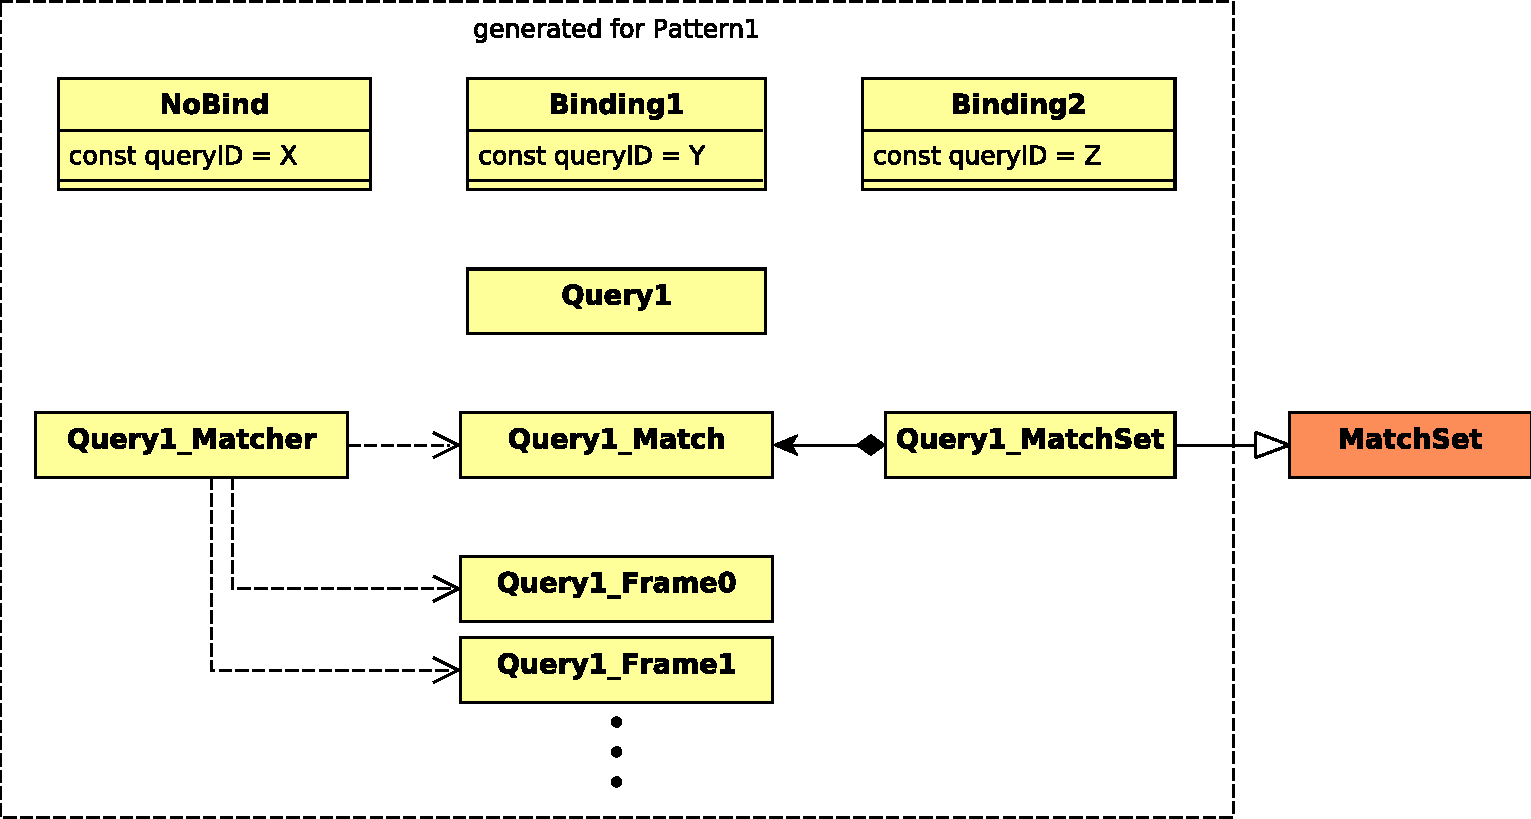
\includegraphics[width=\textwidth]{figures/generated-code-structure-perpattern.pdf}
		\caption{Generated classes for a pattern}
		\label{fig:generated-code-structure-perpattern}
	\end{center}
\end{figure}


\subsection{Integrating with the framework}

\begin{figure}[h]
	\begin{center}
		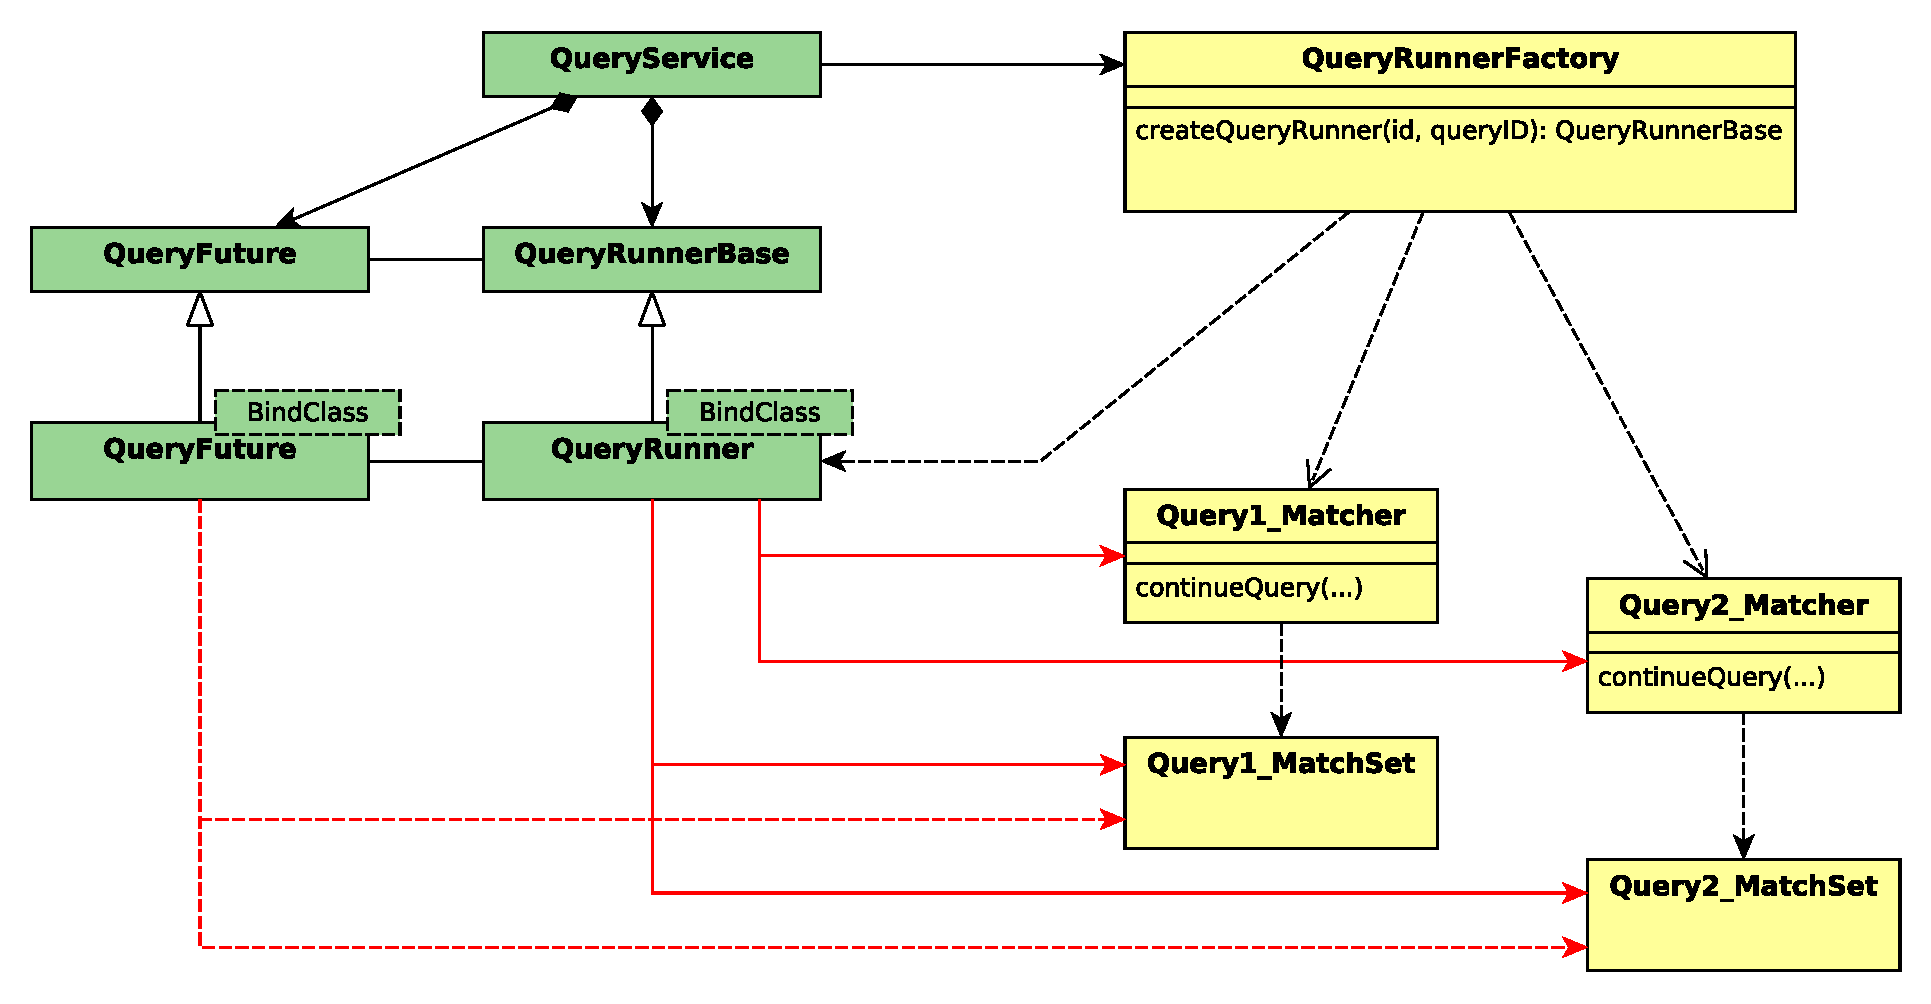
\includegraphics[width=0.9\textwidth]{figures/generated-code-structure-wholesome.pdf}
		\caption{Generated code structure for every pattern}
		\label{fig:generated-code-structure-wholesome}
	\end{center}
\end{figure}

\subsection{Query code generation}

The completed and optimized plan are used to generate \cpp{} code. 
Two main methods can be used to run local search plan in case of generated code. 
One is to generate the plan as a data structure and create an interpreter that uses the plan to find matches. 
The other is to generate the code directly from the plan. 
The first method is good if we want to change the plan at runtime, but the interpreter itself introduces an overhead, causing performance to be slower.
We implemented and measured the performance for both of them.

\todo{Itt konkrétan a kódgenerálás részleteibe bele lehet menni, ha lesz idő}


\subsection{Generating helper data structures}

\subsubsection{Matching frame, frame vector}

The variables of a body are stored in a data structure called the matching frame.
We also generate a collection for frames called frame vector used in distributed behavior of the graph pattern matcher.
We generate serializer and deserializer methods, which uses protobuf.
The message structure (.proto file) is also generated alongside these structures.
\todo{Konkrétan megcsinálni, hogy hogy generálódnak az osztályok, adattagok, névválasztás, XXXMAtchingFrame0, stb}

\subsubsection{Match, MatchSet}

These are used to store graph pattern matches. Match is a singular match (Practically it is the same as the Matching Frame projected to the parameters), while MatchSet is a collection for matches.














%
\chapter{Runtime stuffs}
%



%----------------------------------------------------------------------------
\chapter{Evaluation}
%----------------------------------------------------------------------------


\section{Measurement setup}

To measure the performance of the code generated by our framework we use the following setup. We use 6 BeagleBone Black (BBB) \cite{BBB} as computation units. We connect them via network. 

The model is partitioned to the units in 3 different ways 
\begin{itemize}
	\item Standard -- The model is partitioned by equally distributing the model considering locality ie.\ elements that are connected have more probability of being allocated to the same unit
	\item Alternative -- The model is partitioned by equally distributing the model not considering locality
	\item Single -- All of the elements are allocated on the same node
\end{itemize}

\section{Measurement result}








\section{Evaluation}

\chapter{Conclusions}
\label{sec:conclusion}

In this paper we introduced a novel runtime verification system for distributed CPS systems. The approach is based on the VIATRA-Query graph pattern language, which is used to define analysis properties. Graph models are used to define the structural information captured from the system. A code generator generates the data structures and the code to evaluate the queries on the model at runtime. The model is continuously updated with the information received from the environment and fast query execution provides runtime verification. 
The framework combines various technologies from the model-driven and also the CPS domain into a comprehensive approach. A case-study and measurements are used for evaluation purposes. 
The initial measurements show that the approach is capable of analyzing real life systems and the framework can provide fast results even running in microcomputers with low resources.

In the future we plan to continue this line of research. We hope to extend the model handling to provide more adaptability and new strategies have to be added to efficiently handle highly dynamic systems. In addition, we plan to extend the approach to handle temporal properties.
So there is much work left and there are several points where we can further improve the framework. 


% Acknowledgements
%~~~~~~~~~~~~~~~~~~~~~~~~~~~~~~~~~~~~~~~~~~~~~~~~~~~~~~~~~~~~~~~~~~~~~~~~~~~~~~~~~~~~~~
%%----------------------------------------------------------------------------
\chapter*{\koszonetnyilvanitas}\addcontentsline{toc}{chapter}{\koszonetnyilvanitas}
%----------------------------------------------------------------------------



% List of Figures, Tables
%~~~~~~~~~~~~~~~~~~~~~~~~~~~~~~~~~~~~~~~~~~~~~~~~~~~~~~~~~~~~~~~~~~~~~~~~~~~~~~~~~~~~~~
%\listoffigures\addcontentsline{toc}{chapter}{\listfigurename}
%\listoftables\addcontentsline{toc}{chapter}{\listtablename}


% Bibliography
%~~~~~~~~~~~~~~~~~~~~~~~~~~~~~~~~~~~~~~~~~~~~~~~~~~~~~~~~~~~~~~~~~~~~~~~~~~~~~~~~~~~~~~
\bibliography{bib/mybib}
\addcontentsline{toc}{chapter}{\bibname}


% Appendix
%~~~~~~~~~~~~~~~~~~~~~~~~~~~~~~~~~~~~~~~~~~~~~~~~~~~~~~~~~~~~~~~~~~~~~~~~~~~~~~~~~~~~~~
%----------------------------------------------------------------------------
\appendix
%----------------------------------------------------------------------------
\chapter*{\fuggelek}\addcontentsline{toc}{chapter}{\fuggelek}
\setcounter{chapter}{\appendixnumber}
%\setcounter{equation}{0} % a fofejezet-szamlalo az angol ABC 6. betuje (F) lesz
\numberwithin{equation}{section}
\numberwithin{figure}{section}
\numberwithin{lstlisting}{section}
%\numberwithin{tabular}{section}

%----------------------------------------------------------------------------
\section{Measured queries}
%----------------------------------------------------------------------------


\subsection{Benchmarked patterns}

\begin{lstlisting}[language = vql]
pattern trainLocations(train: Train, loc: RailRoadElement)
{
	Train.on(train, loc);
}
\end{lstlisting}

\begin{lstlisting}[language = vql]
pattern derailment(elem: RailRoadElement, train: Train)
{
	Turnout(turnout);
	RailRoadElement.train(elem,train);
	
	neg find connected(elem, turnout);
	find straightOrDivergent(turnout, elem);
}
\end{lstlisting}

\begin{lstlisting}[language = vql]
pattern CloseTrains(start : RailRoadElement, end : RailRoadElement)
{
	
	Train.on(t1,start);
	
	RailRoadElement.connectedTo(start,middle); // Has EOpposite, inverse navigation is effective even without model index
	RailRoadElement.connectedTo(middle, end);
	
	start != end; // This ensures that at least the start and end segment is different
	
	RailRoadElement.train(end, t2);
	
	t1 != t2; // A train may occupy two neighboring segments when moving; this is not a hazardous situation
	
	// Allocation-specific part of the query: global or local execution is based on the substitutions of c1 and c2
}
\end{lstlisting}

\begin{lstlisting}[language = vql]
pattern endOfSiding(train: Train, end: RailRoadElement, neighbor: RailRoadElement)
{
	RailRoadElement.connectedTo(end,neighbor);
	neg find otherNeighbor(end,neighbor,_);
	
	RailRoadElement.train(neighbor, train);	
}
\end{lstlisting}

\clearpage

\subsection{Helper patterns for benchmark patterns}


\begin{lstlisting}[language = vql]
private pattern connected(a : RailRoadElement, b : RailRoadElement){
	RailRoadElement.connectedTo(a,b);
}
\end{lstlisting}

\begin{lstlisting}[language = vql]
private pattern straightOrDivergent(turnout : Turnout, elem : RailRoadElement){
	Turnout.straight(turnout, elem);
} or {
	Turnout.divergent(turnout, elem);
}
\end{lstlisting}

\begin{lstlisting}[language = vql]
private pattern otherNeighbor(e : RailRoadElement, n1 : RailRoadElement, n2 : RailRoadElement){	
	RailRoadElement.connectedTo(e,n1);
	RailRoadElement.connectedTo(e,n2);
	n1 != n2;
}

\end{lstlisting}

\vfill

%----------------------------------------------------------------------------
%\clearpage\section{Measured queries}
%----------------------------------------------------------------------------



%\label{page:last}
\end{document}
